% !TeX program = xelatex
\documentclass[11pt,a4paper]{article}

% -------------------------------------------------
% Packages
% -------------------------------------------------
\usepackage{kotex}
\usepackage{fontspec}
\usepackage{amsmath,amssymb,bm,mathtools}
\usepackage[left=24mm,right=24mm,top=23mm,bottom=25mm]{geometry}
\usepackage{booktabs,array}
\usepackage{enumitem}
\usepackage{setspace}
\usepackage{xcolor}
\usepackage{colortbl}
\usepackage{tikz}
\usepackage{pifont}
\usetikzlibrary{positioning,arrows.meta,calc,fit,decorations.pathreplacing}
\usepackage[most]{tcolorbox}
\usepackage{listings}
\usepackage{hyperref}
\usepackage{fancyhdr}

\setstretch{1.14}
\setlength{\parindent}{0pt}
\setlength{\parskip}{0.55em}

% -------------------------------------------------
% Colors and boxes
% -------------------------------------------------
\definecolor{deepblue}{RGB}{34,71,120}
\definecolor{softblue}{RGB}{239,246,253}
\definecolor{softgray}{RGB}{246,247,249}
\definecolor{softgreen}{RGB}{239,249,242}
\definecolor{softyellow}{RGB}{255,249,229}
\definecolor{codegray}{RGB}{248,248,248}

\newtcolorbox{keybox}[1][]{
  colback=softblue,
  colframe=deepblue,
  boxrule=0.7pt,
  arc=2mm,
  title=#1,
  fonttitle=\bfseries
}

\newtcolorbox{thinkbox}[1][]{
  colback=softyellow,
  colframe=orange!70!black,
  boxrule=0.6pt,
  arc=2mm,
  title=#1,
  fonttitle=\bfseries
}

\newtcolorbox{remarkbox}[1][]{
  colback=softgray,
  colframe=black!45,
  boxrule=0.5pt,
  arc=2mm,
  title=#1,
  fonttitle=\bfseries
}

\newtcolorbox{mlbox}[1][]{
  colback=softgreen,
  colframe=green!45!black,
  boxrule=0.6pt,
  arc=2mm,
  title=#1,
  fonttitle=\bfseries
}

% -------------------------------------------------
% Code style
% -------------------------------------------------
\lstdefinestyle{pythonstyle}{
  language=Python,
  backgroundcolor=\color{codegray},
  basicstyle=\ttfamily\small,
  keywordstyle=\bfseries,
  commentstyle=\itshape\color{black!60},
  stringstyle=\color{black!75},
  numbers=left,
  numberstyle=\tiny\color{black!55},
  numbersep=8pt,
  frame=single,
  rulecolor=\color{black!25},
  breaklines=true,
  showstringspaces=false,
  tabsize=4,
  columns=fullflexible,
  keepspaces=true
}
\lstset{style=pythonstyle}

% -------------------------------------------------
% Math commands
% -------------------------------------------------
\newcommand{\R}{\mathbb{R}}
\newcommand{\grad}{\nabla}
\newcommand{\vect}[1]{\bm{#1}}
\newcommand{\T}{^{\mathsf T}}
\newcommand{\loss}{\mathcal{L}}
\newcommand{\sigmoid}{\sigma}
\newcommand{\pd}[2]{\frac{\partial #1}{\partial #2}}
\newcommand{\softmax}{\operatorname{softmax}}

% -------------------------------------------------
% Header / footer
% -------------------------------------------------
\pagestyle{fancy}
\fancyhf{}
\lhead{Introduction to Deep Learning and Practice}
\rhead{Convolutional Neural Networks}
\cfoot{\thepage}
\renewcommand{\headrulewidth}{0.4pt}
\setlength{\headheight}{14pt}

\hypersetup{
  colorlinks=true,
  linkcolor=deepblue,
  urlcolor=deepblue
}

% =================================================
% =================================================
\begin{document}
% =================================================

% ---- drawing helpers for this chapter ----
\def\cellsz{0.5}% size of one cell in the grid figures (cm)
% \numgrid{x}{y}{columns}{list}: a grid of numbers, top-left corner at (x, y)
\newcommand{\numgrid}[4]{%
  \foreach \v [count=\k from 0] in {#4} {%
    \pgfmathtruncatemacro{\rr}{int(\k/#3)}%
    \pgfmathtruncatemacro{\cc}{mod(\k,#3)}%
    \draw[black!55] ({#1+\cc*\cellsz},{#2-\rr*\cellsz}) rectangle ++(\cellsz,-\cellsz);%
    \node[font=\small] at ({#1+\cc*\cellsz+0.5*\cellsz},{#2-\rr*\cellsz-0.5*\cellsz}) {\v};%
  }}
% \cuboid{x}{y}{width}{height}{depth}{color}: a block, front face bottom-left at (x, y)
\newcommand{\cuboid}[6]{%
  \filldraw[fill=#6!25,draw=black!70] ({#1},{#2}) rectangle ++({#3},{#4});%
  \filldraw[fill=#6!40,draw=black!70] ({#1},{#2+#4}) -- ++({0.5*#5},{0.4*#5}) -- ++({#3},0) -- ++({-0.5*#5},{-0.4*#5}) -- cycle;%
  \filldraw[fill=#6!55,draw=black!70] ({#1+#3},{#2}) -- ++({0.5*#5},{0.4*#5}) -- ++(0,{#4}) -- ++({-0.5*#5},{-0.4*#5}) -- cycle;%
}

\begin{center}
{\LARGE\bfseries 합성곱 신경망 (CNN)}\\[0.35em]
{\large 합성곱 계층 $\cdot$ 풀링 계층 $\cdot$ im2col $\cdot$ SimpleConvNet $\cdot$ LeNet과 AlexNet}\\[0.8em]
\end{center}

\vspace{0.4em}

\begin{keybox}[이번 주의 핵심 질문]
지금까지의 신경망은 MNIST의 $28\times28$ 이미지를 길이 $784$의 벡터로 \textbf{펼쳐서} 입력하였다.
그러면 ``이 픽셀의 바로 위와 바로 옆에 어떤 픽셀이 있는가''라는 \textbf{공간 정보}가 사라진다.
이미지의 모양을 그대로 유지한 채 학습하는 방법은 없을까?
그리고 이미지의 어느 위치에 있든 같은 모양(예: 세로 획)을 같은 방법으로 알아보려면 어떻게 해야 할까?
\end{keybox}

\subsection*{학습목표}

이 주차가 끝나면 다음을 설명하고 직접 계산할 수 있어야 한다.

\begin{enumerate}[label=\arabic*.]
\item 완전연결 계층과 비교하여 합성곱 계층이 이미지에 적합한 이유(공간 정보, 가중치 공유)를 설명한다.
\item 합성곱 연산을 손으로 계산하고, 패딩과 스트라이드에 따른 출력 크기를 구한다.
\item 여러 채널, 여러 필터, 미니배치에 대한 합성곱을 4차원 배열의 shape으로 설명한다.
\item 최대 풀링의 계산과 그 특징을 설명한다.
\item im2col을 이용하여 합성곱을 하나의 행렬곱(Affine 계층)으로 바꾸고, 그 역전파를 유도한다.
\item 합성곱 계층과 풀링 계층으로 CNN을 구성하여 MNIST를 학습시키고, 학습된 필터를 해석한다.
\item LeNet과 AlexNet의 구조와 차이를 설명한다.
\end{enumerate}

% =================================================
\section{전체 구조}\label{sec:structure}
% =================================================

\textbf{합성곱 신경망(Convolutional Neural Network, CNN)}은 이미지 인식과 음성 인식 등 다양한 곳에서 쓰이는 신경망이다.
지금까지 본 신경망과 마찬가지로 계층을 조합하여 만들지만,
\textbf{합성곱 계층(convolutional layer)}과 \textbf{풀링 계층(pooling layer)}이라는 새로운 계층이 등장한다.

지금까지의 신경망은 인접하는 계층의 모든 node가 연결되어 있었다.
이것을 \textbf{완전연결(fully-connected)}이라 하며, 완전연결 계층을 Affine 계층이라는 이름으로 구현하였다.

\begin{center}
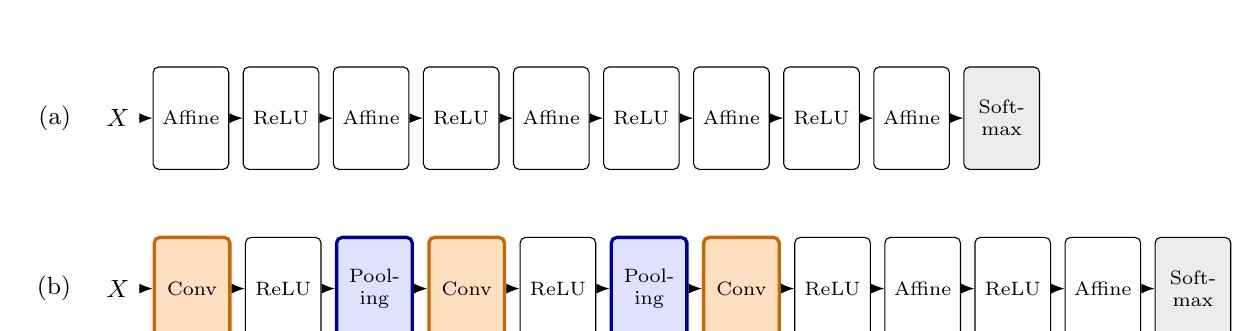
\begin{tikzpicture}[>=Latex,
  lay/.style={draw,rounded corners=2pt,minimum width=9.6mm,minimum height=13mm,
              font=\scriptsize,align=center,inner sep=1pt},
  cv/.style={lay,fill=orange!25,draw=orange!80!black,very thick},
  pl/.style={lay,fill=blue!12,draw=blue!60!black,very thick},
  node distance=1.7mm]
% fully connected
\node[font=\small] (in) {$X$};
\node[lay,right=of in] (a1) {Affine};
\node[lay,right=of a1] (r1) {ReLU};
\node[lay,right=of r1] (a2) {Affine};
\node[lay,right=of a2] (r2) {ReLU};
\node[lay,right=of r2] (a3) {Affine};
\node[lay,right=of a3] (r3) {ReLU};
\node[lay,right=of r3] (a4) {Affine};
\node[lay,right=of a4] (r4) {ReLU};
\node[lay,right=of r4] (a5) {Affine};
\node[lay,right=of a5,fill=black!8] (sm) {Soft-\\max};
\foreach \u/\v in {in/a1,a1/r1,r1/a2,a2/r2,r2/a3,a3/r3,r3/a4,a4/r4,r4/a5,a5/sm}
  \draw[->] (\u) -- (\v);
\node[font=\small,anchor=east] at ([xshift=-2mm]in.west) {(a)};
% CNN
\node[font=\small,below=17mm of in] (in2) {$X$};
\node[cv,right=of in2] (c1) {Conv};
\node[lay,right=of c1] (q1) {ReLU};
\node[pl,right=of q1] (p1) {Pool-\\ing};
\node[cv,right=of p1] (c2) {Conv};
\node[lay,right=of c2] (q2) {ReLU};
\node[pl,right=of q2] (p2) {Pool-\\ing};
\node[cv,right=of p2] (c3) {Conv};
\node[lay,right=of c3] (q3) {ReLU};
\node[lay,right=of q3] (b1) {Affine};
\node[lay,right=of b1] (s1) {ReLU};
\node[lay,right=of s1] (b2) {Affine};
\node[lay,right=of b2,fill=black!8] (sm2) {Soft-\\max};
\foreach \u/\v in {in2/c1,c1/q1,q1/p1,p1/c2,c2/q2,q2/p2,p2/c3,c3/q3,q3/b1,b1/s1,s1/b2,b2/sm2}
  \draw[->] (\u) -- (\v);
\node[font=\small,anchor=east] at ([xshift=-2mm]in2.west) {(b)};
\end{tikzpicture}

\small (a) 완전연결 계층(Affine)으로 이루어진 신경망. (b) CNN의 예:
주황색이 합성곱 계층(Conv), 파란색이 풀링 계층(Pooling)이다.
\end{center}

CNN에서는 ``Affine $\to$ ReLU'' 대신 ``Conv $\to$ ReLU $\to$ (Pooling)''의 흐름이 이어진다
(풀링 계층은 생략하기도 한다).
출력에 가까운 층에서는 지금까지의 ``Affine $\to$ ReLU''를 쓰고, 마지막은 ``Affine $\to$ Softmax''이다.
즉 CNN은 앞부분에서 이미지의 특징을 뽑고, 뒷부분은 지금까지의 신경망으로 분류하는 구조이다.

% =================================================
\section{합성곱 계층}\label{sec:conv}
% =================================================

\subsection{완전연결 계층의 문제점}\label{sec:fcproblem}

완전연결 계층의 문제점은 \textbf{데이터의 형상이 무시된다}는 것이다.
MNIST 이미지는 세로 $28$, 가로 $28$, 채널 $1$ (흑백)인 3차원 데이터 $(1, 28, 28)$이지만,
Affine 계층에 넣으려면 $784$개의 값을 한 줄로 펼쳐야 했다.
이미지에서는 공간적으로 가까운 픽셀끼리 값이 비슷하고, RGB의 세 채널은 서로 밀접하게 관련되어 있으며,
떨어진 픽셀끼리는 관련이 적다. 이런 \textbf{3차원 모양에 담긴 패턴}이 펼치는 순간 사라진다.
완전연결 계층은 모든 입력을 같은 차원의 값으로 취급하므로, 픽셀의 순서를 무작위로 섞어도 학습 결과가 똑같다.

합성곱 계층은 이 \textbf{형상을 유지}한다. 이미지를 3차원 데이터로 입력받고, 다음 계층에도 3차원 데이터로 전달한다.
CNN에서 합성곱 계층의 입출력 데이터를 \textbf{특징 맵(feature map)}이라 한다.
입력 데이터를 \textbf{입력 특징 맵}, 출력 데이터를 \textbf{출력 특징 맵}이라 부른다.

\subsection{합성곱 연산}\label{sec:convop}

합성곱 계층에서는 \textbf{합성곱 연산}을 한다. 이미지 처리에서 말하는 \textbf{필터 연산}이다.
먼저 채널이 하나인 경우를 보자. 입력은 $(4,4)$, 필터는 $(3,3)$이다.
필터를 \textbf{커널(kernel)}이라고도 한다.

\begin{center}
\begin{tikzpicture}
\numgrid{0}{0}{4}{1,2,3,0,0,1,2,3,3,0,1,2,2,3,0,1}
\node[font=\Large] at (2.55,-1) {$\circledast$};
\numgrid{3.1}{-0.25}{3}{2,0,1,0,1,2,1,0,2}
\node[font=\Large] at (5.15,-1) {$\longrightarrow$};
\numgrid{5.8}{-0.5}{2}{15,16,6,15}
\node[font=\small,below] at (1,-2.1) {입력 데이터};
\node[font=\small,below] at (3.85,-2.1) {필터};
\node[font=\small,below] at (6.3,-2.1) {출력};
\end{tikzpicture}
\end{center}

합성곱 연산은 필터의 \textbf{윈도우(window)}를 일정 간격으로 이동해 가며 입력 데이터에 적용한다.
각 위치에서 입력과 필터의 \textbf{대응하는 원소끼리 곱한 뒤 모두 더한다} (단일 곱셈-누산, fused multiply-add).
그 결과를 출력의 해당 위치에 저장한다. 왼쪽 위부터 오른쪽 아래까지 모든 위치에서 이 계산을 반복한다.

\begin{center}
\begin{tikzpicture}
\foreach \oi/\oj/\px/\py/\val in {0/0/0/0/15, 0/1/7.6/0/16, 1/0/0/-3.1/6, 1/1/7.6/-3.1/15} {
  \begin{scope}[shift={(\px,\py)}]
    \fill[orange!30] ({\oj*\cellsz},{-\oi*\cellsz}) rectangle ++({3*\cellsz},{-3*\cellsz});
    \numgrid{0}{0}{4}{1,2,3,0,0,1,2,3,3,0,1,2,2,3,0,1}
    \draw[orange!80!black,very thick] ({\oj*\cellsz},{-\oi*\cellsz}) rectangle ++({3*\cellsz},{-3*\cellsz});
    \node at (2.4,-1) {$\circledast$};
    \numgrid{2.85}{-0.25}{3}{2,0,1,0,1,2,1,0,2}
    \node at (4.75,-1) {$\to$};
    \fill[orange!30] ({5.1+\oj*\cellsz},{-0.5-\oi*\cellsz}) rectangle ++(\cellsz,-\cellsz);
    \draw[orange!80!black,very thick] ({5.1+\oj*\cellsz},{-0.5-\oi*\cellsz}) rectangle ++(\cellsz,-\cellsz);
    \draw[black!55] (5.1,-0.5) grid[step=\cellsz] ++({2*\cellsz},{-2*\cellsz});
    \node[font=\small] at ({5.1+\oj*\cellsz+0.5*\cellsz},{-0.5-\oi*\cellsz-0.5*\cellsz}) {\val};
  \end{scope}
}
\end{tikzpicture}

\small 합성곱 연산의 계산 순서. 주황색 윈도우가 왼쪽 위에서 오른쪽 아래로 이동한다.
\end{center}
예를 들어 첫 번째 위치에서는
\[
1\cdot2+2\cdot0+3\cdot1+0\cdot0+1\cdot1+2\cdot2+3\cdot1+0\cdot0+1\cdot2=15
\]
이다. 식으로 쓰면, 입력 $x$와 필터 $f$ ($FH\times FW$)에 대하여 출력의 $(i,j)$ 원소는
\[
y_{ij}=\sum_{p=0}^{FH-1}\sum_{q=0}^{FW-1}x_{i+p,\,j+q}\,f_{pq}
\]
이다.

\paragraph{필터가 가중치이다.}
완전연결 신경망에는 가중치 $W$와 편향 $B$가 있었다.
CNN에서는 \textbf{필터의 원소가 가중치}에 해당한다. 필터의 값을 학습하는 것이다.
편향은 필터를 적용한 뒤 모든 원소에 같은 값 하나를 더한다.

\begin{center}
\begin{tikzpicture}
\numgrid{0}{0}{4}{1,2,3,0,0,1,2,3,3,0,1,2,2,3,0,1}
\node[font=\Large] at (2.5,-1) {$\circledast$};
\numgrid{3.0}{-0.25}{3}{2,0,1,0,1,2,1,0,2}
\node[font=\Large] at (5.0,-1) {$\to$};
\numgrid{5.5}{-0.5}{2}{15,16,6,15}
\node[font=\Large] at (7.0,-1) {$+$};
\numgrid{7.5}{-0.75}{1}{3}
\node[font=\Large] at (8.5,-1) {$\to$};
\numgrid{9.0}{-0.5}{2}{18,19,9,18}
\node[font=\small,below] at (3.75,-1.9) {필터 (가중치)};
\node[font=\small,below] at (7.75,-1.9) {편향};
\end{tikzpicture}
\end{center}

\begin{remarkbox}[합성곱(convolution)과 상호상관(cross-correlation)]
수학과 신호처리에서 말하는 합성곱은 필터를 상하좌우로 \textbf{뒤집은 뒤} 곱하고 더한다
($y_{ij}=\sum x_{i-p,\,j-q}f_{pq}$). 위의 연산처럼 뒤집지 않는 것은 원래 \textbf{상호상관}이라고 부른다.
그러나 필터는 어차피 학습되는 값이므로 뒤집든 안 뒤집든 학습 결과는 같은 것을 표현할 수 있다.
그래서 딥러닝에서는 뒤집지 않는 연산을 관례적으로 ``합성곱''이라 부르며, PyTorch의 \texttt{nn.Conv2d}도 뒤집지 않는다.
\end{remarkbox}

\paragraph{코드로 확인하기.}
\texttt{conv\_basics.py}에서 채널 하나, 필터 하나인 합성곱을 반복문으로 쓰면 다음과 같다.
\begin{lstlisting}
def conv2d_naive(x, f, stride=1, pad=0):
    """2-D convolution of one image x (H, W) with one filter f (FH, FW), with loops"""
    x = np.pad(x, pad)                                  # zeros around the image
    FH, FW = f.shape
    OH = (x.shape[0] - FH) // stride + 1
    OW = (x.shape[1] - FW) // stride + 1
    y = np.zeros((OH, OW))
    for i in range(OH):
        for j in range(OW):
            window = x[i * stride:i * stride + FH, j * stride:j * stride + FW]
            y[i, j] = np.sum(window * f)                # multiply elementwise, then add
    return y
\end{lstlisting}
\begin{lstlisting}
print("convolution (4x4 input, 3x3 filter):\n", conv2d_naive(x, f))
print("with bias 3:\n", conv2d_naive(x, f) + 3)
print("padding 1:\n", conv2d_naive(x, f, pad=1))
\end{lstlisting}
\begin{lstlisting}[language={},numbers=none]
convolution (4x4 input, 3x3 filter):
 [[15. 16.]
 [ 6. 15.]]
with bias 3:
 [[18. 19.]
 [ 9. 18.]]
\end{lstlisting}

\subsection{패딩}\label{sec:padding}

합성곱 연산을 하기 전에 입력 데이터 주변을 특정 값(보통 $0$)으로 채우기도 한다.
이것을 \textbf{패딩(padding)}이라 한다. 아래는 $(4,4)$ 입력에 폭 $1$의 패딩을 적용한 예이다.

\begin{center}
\begin{tikzpicture}
\fill[black!8] (0,0) rectangle ({6*\cellsz},{-6*\cellsz});
\numgrid{0}{0}{6}{0,0,0,0,0,0,0,1,2,3,0,0,0,0,1,2,3,0,0,3,0,1,2,0,0,2,3,0,1,0,0,0,0,0,0,0}
\draw[very thick] (\cellsz,-\cellsz) rectangle ({5*\cellsz},{-5*\cellsz});
\node[font=\Large] at (3.45,-1.5) {$\circledast$};
\numgrid{4.0}{-0.75}{3}{2,0,1,0,1,2,1,0,2}
\node[font=\Large] at (6.05,-1.5) {$\longrightarrow$};
\numgrid{6.7}{-0.5}{4}{7,12,10,2,4,15,16,10,10,6,15,6,8,10,4,3}
\node[font=\small,below] at (1.5,-3.1) {$(4,4)$ 입력 + 패딩 $1$};
\node[font=\small,below] at (4.75,-3.1) {$(3,3)$ 필터};
\node[font=\small,below] at (7.7,-3.1) {$(4,4)$ 출력};
\end{tikzpicture}
\end{center}

패딩이 없으면 $(4,4)$ 입력이 $(2,2)$로 줄어들지만, 패딩을 $1$ 하면 출력도 $(4,4)$로 입력과 같은 크기가 된다.
\begin{lstlisting}[language={},numbers=none]
padding 1:
 [[ 7. 12. 10.  2.]
 [ 4. 15. 16. 10.]
 [10.  6. 15.  6.]
 [ 8. 10.  4.  3.]]
\end{lstlisting}
패딩은 주로 \textbf{출력 크기를 조정}하려고 쓴다.
합성곱 연산을 할 때마다 크기가 줄어들면, 합성곱을 여러 번 거치는 깊은 network에서는 어느 시점에 출력이 $1$이 되어
더 이상 합성곱을 할 수 없게 된다. 패딩을 쓰면 공간 크기를 유지한 채 다음 계층에 전달할 수 있다.
또 패딩이 없으면 가장자리의 픽셀은 필터가 몇 번밖에 지나가지 않아 정보가 덜 반영된다.

\subsection{스트라이드}\label{sec:stride}

필터를 적용하는 위치의 간격을 \textbf{스트라이드(stride)}라 한다. 지금까지는 스트라이드가 $1$이었다.
스트라이드를 $2$로 하면 윈도우가 두 칸씩 이동한다.

\begin{center}
\begin{tikzpicture}
\fill[orange!30] (0,0) rectangle ({3*\cellsz},{-3*\cellsz});
\fill[blue!15] ({2*\cellsz},0) rectangle ({5*\cellsz},{-3*\cellsz});
\fill[orange!55!blue!30] ({2*\cellsz},0) rectangle ({3*\cellsz},{-3*\cellsz});
\draw[black!55] (0,0) grid[step=\cellsz] ({7*\cellsz},{-7*\cellsz});
\draw[orange!80!black,very thick] (0,0) rectangle ({3*\cellsz},{-3*\cellsz});
\draw[blue!70!black,very thick,densely dashed] ({2*\cellsz},0) rectangle ({5*\cellsz},{-3*\cellsz});
\draw[->,thick] (0.75,0.35) -- node[above,font=\small] {스트라이드 $2$} (1.75,0.35);
\node[font=\Large] at (4.2,-1.75) {$\circledast$};
\draw[black!55] (4.75,-1) grid[step=\cellsz] ++({3*\cellsz},{-3*\cellsz});
\node[font=\Large] at (7,-1.75) {$\longrightarrow$};
\fill[orange!30] (7.6,-1) rectangle ++(\cellsz,-\cellsz);
\fill[blue!15] ({7.6+\cellsz},-1) rectangle ++(\cellsz,-\cellsz);
\draw[black!55] (7.6,-1) grid[step=\cellsz] ++({3*\cellsz},{-3*\cellsz});
\node[font=\small,below] at (1.75,-3.6) {$(7,7)$ 입력};
\node[font=\small,below] at (5.5,-3.6) {$(3,3)$ 필터};
\node[font=\small,below] at (8.35,-3.6) {$(3,3)$ 출력};
\end{tikzpicture}
\end{center}

스트라이드를 키우면 출력이 작아지고, 패딩을 키우면 출력이 커진다.
입력 크기를 $(H,W)$, 필터 크기를 $(FH,FW)$, 패딩을 $P$, 스트라이드를 $S$라 하면 출력 크기 $(OH,OW)$는

\begin{keybox}[합성곱의 출력 크기]
\[
OH=\frac{H+2P-FH}{S}+1,\qquad OW=\frac{W+2P-FW}{S}+1
\]
\end{keybox}

이다. 예를 들어
\begin{itemize}[leftmargin=1.8em]
\item 입력 $(4,4)$, 패딩 $1$, 스트라이드 $1$, 필터 $(3,3)$: $OH=\frac{4+2-3}{1}+1=4$
\item 입력 $(7,7)$, 패딩 $0$, 스트라이드 $2$, 필터 $(3,3)$: $OH=\frac{7+0-3}{2}+1=3$
\item 입력 $(28,31)$, 패딩 $2$, 스트라이드 $3$, 필터 $(5,5)$: $OH=\frac{28+4-5}{3}+1=10$, $OW=\frac{31+4-5}{3}+1=11$
\end{itemize}
이 식이 정수로 나누어떨어지도록 값을 정해야 한다. 나누어떨어지지 않으면 오류를 내거나,
프레임워크에 따라 가장 가까운 정수로 반올림하는 등 별도로 처리한다.
\begin{lstlisting}[language={},numbers=none]
7x7 input, 3x3 filter, stride 1 -> shape (5, 5)
7x7 input, 3x3 filter, stride 2 -> shape (3, 3)
\end{lstlisting}

\subsection{3차원 데이터의 합성곱}\label{sec:conv3d}

이미지는 보통 세로, 가로에 \textbf{채널} 방향까지 있는 3차원 데이터이다 (컬러 이미지는 RGB의 $3$채널).
채널이 여러 개이면 \textbf{채널마다 입력과 필터의 합성곱}을 하고, 그 결과를 \textbf{모두 더해서} 하나의 출력을 얻는다.

\begin{center}
\begin{tikzpicture}
\foreach \c/\col in {2/blue,1/green!60!black,0/orange} {
  \begin{scope}[shift={({0.3*\c},{0.3*\c})}]
    \filldraw[fill=\col!15,draw=black!60] (0,0) rectangle ({4*\cellsz},{-4*\cellsz});
    \draw[black!40] (0,0) grid[step=\cellsz] ({4*\cellsz},{-4*\cellsz});
  \end{scope}
  \begin{scope}[shift={({3.3+0.3*\c},{-0.25+0.3*\c})}]
    \filldraw[fill=\col!15,draw=black!60] (0,0) rectangle ({3*\cellsz},{-3*\cellsz});
    \draw[black!40] (0,0) grid[step=\cellsz] ({3*\cellsz},{-3*\cellsz});
  \end{scope}
}
\node[font=\Large] at (2.75,-1) {$\circledast$};
\node[font=\Large] at (5.6,-1) {$\longrightarrow$};
\filldraw[fill=black!8,draw=black!60] (6.3,-0.5) rectangle ++({2*\cellsz},{-2*\cellsz});
\draw[black!40] (6.3,-0.5) grid[step=\cellsz] ++({2*\cellsz},{-2*\cellsz});
\node[font=\small,below,align=center] at (1.3,-2.15) {입력 데이터\\(채널 $3$개, $4\times4$)};
\node[font=\small,below,align=center] at (4.1,-2.15) {필터\\(채널 $3$개, $3\times3$)};
\node[font=\small,below,align=center] at (6.8,-2.15) {출력\\($2\times2$, 채널 $1$개)};
\end{tikzpicture}
\end{center}

\begin{keybox}[3차원 합성곱의 규칙]
\textbf{입력 데이터의 채널 수와 필터의 채널 수가 같아야 한다.}
필터의 크기 $(FH,FW)$는 원하는 값으로 정할 수 있지만, 모든 채널의 필터는 같은 크기여야 한다.
채널 $C$개인 입력에 필터 하나를 적용하면 출력은 \textbf{채널 $1$개}의 특징 맵이 된다.
\[
y_{ij}=\sum_{c=1}^{C}\sum_{p}\sum_{q}x_{c,\,i+p,\,j+q}\,f_{c,\,p,\,q}+b
\]
\end{keybox}

\subsection{블록으로 생각하기}\label{sec:blocks}

3차원 합성곱은 데이터와 필터를 직육면체 \textbf{블록}으로 생각하면 이해하기 쉽다.
3차원 데이터의 shape을 (채널, 높이, 너비) $=(C,H,W)$ 순서로 쓴다.
필터는 $(C,FH,FW)$이다.

\begin{center}
\begin{tikzpicture}
\cuboid{0}{0}{1.6}{1.6}{0.9}{blue}
\node[font=\small,below] at (0.8,-0.05) {$(C,H,W)$};
\node[font=\small] at (2.45,0.8) {$\circledast$};
\cuboid{2.9}{0.35}{0.9}{0.9}{0.9}{blue}
\node[font=\small,below] at (3.35,0.3) {$(C,FH,FW)$};
\node[font=\small] at (4.75,0.8) {$\longrightarrow$};
\cuboid{5.3}{0.2}{1.2}{1.2}{0.12}{orange}
\node[font=\small,below] at (5.9,0.15) {$(1,OH,OW)$};
\node[font=\small,anchor=west] at (7.3,0.8) {필터 $1$개 $\Rightarrow$ 특징 맵 $1$장};
\end{tikzpicture}
\end{center}

출력이 한 장(채널 $1$개)이면 다음 계층에 넘길 정보가 너무 적다.
\textbf{필터를 $FN$개} 쓰면 출력 특징 맵도 $FN$장이 되어 $(FN,OH,OW)$ 블록이 된다.
따라서 합성곱 계층의 필터(가중치)는 \textbf{4차원} $(FN,C,FH,FW)$이고,
편향은 필터마다 하나씩 $FN$개이다 (shape $(FN,1,1)$로 보면 broadcast로 더해진다).

\begin{center}
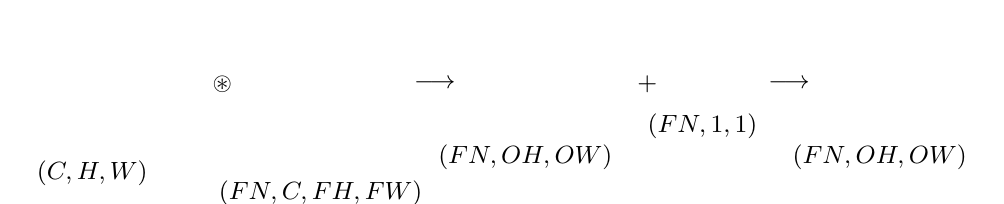
\begin{tikzpicture}
\cuboid{0}{0}{1.6}{1.6}{0.9}{blue}
\node[font=\small,below] at (0.8,-0.05) {$(C,H,W)$};
\node[font=\small] at (2.45,0.8) {$\circledast$};
\foreach \k in {3,2,1,0} {\cuboid{2.9+0.25*\k}{0.35-0.2*\k}{0.8}{0.8}{0.7}{blue}}
\node[font=\small,below] at (3.7,-0.3) {$(FN,C,FH,FW)$};
\node[font=\small] at (5.15,0.8) {$\longrightarrow$};
\cuboid{5.7}{0.2}{1.2}{1.2}{0.8}{orange}
\node[font=\small,below] at (6.3,0.15) {$(FN,OH,OW)$};
\node[font=\small] at (7.85,0.8) {$+$};
\cuboid{8.3}{0.65}{0.25}{0.25}{0.8}{orange}
\node[font=\small,below] at (8.55,0.55) {$(FN,1,1)$};
\node[font=\small] at (9.65,0.8) {$\longrightarrow$};
\cuboid{10.2}{0.2}{1.2}{1.2}{0.8}{orange}
\node[font=\small,below] at (10.8,0.15) {$(FN,OH,OW)$};
\end{tikzpicture}

\small 필터 $FN$개를 쓰는 합성곱 계층. 편향은 필터(출력 채널)마다 하나이다.
\end{center}

\begin{thinkbox}[왜 합성곱인가: 가중치 공유]
합성곱 계층에서는 \textbf{같은 필터를 이미지의 모든 위치에 적용}한다 (가중치 공유, weight sharing).
그래서 세로 획을 찾는 필터 하나가 이미지의 왼쪽 위에 있는 세로 획과 오른쪽 아래에 있는 세로 획을 똑같이 찾아낸다.
또 매개변수가 아주 적다. MNIST 이미지 $(1,28,28)$에서 $(30,24,24)$의 출력을 만든다고 하자.
\begin{itemize}[leftmargin=1.5em]
\item 완전연결 계층: $784\times(30\cdot24\cdot24)=784\times17280\approx1350$만 개의 가중치
\item 합성곱 계층 ($5\times5$ 필터 $30$개): $30\times1\times5\times5=750$개의 가중치와 $30$개의 편향
\end{itemize}
각 출력 원소는 입력의 $5\times5$ 영역만 본다 (\textbf{국소 연결}). 이 두 성질이 이미지의 구조에 잘 맞는다.
\end{thinkbox}

\subsection{배치 처리}\label{sec:convbatch}

완전연결 계층에서 미니배치로 데이터를 묶어 한 번에 처리했듯이, 합성곱 계층도 배치 처리를 한다.
각 계층을 흐르는 데이터에 차원을 하나 더 늘려 \textbf{4차원} (데이터 수, 채널, 높이, 너비) $=(N,C,H,W)$로 저장한다.
(지금까지 미니배치 크기를 $h$라 했지만, 이 장에서는 높이 $H$와 헷갈리지 않도록 책처럼 $N$이라 쓴다.)

\begin{center}
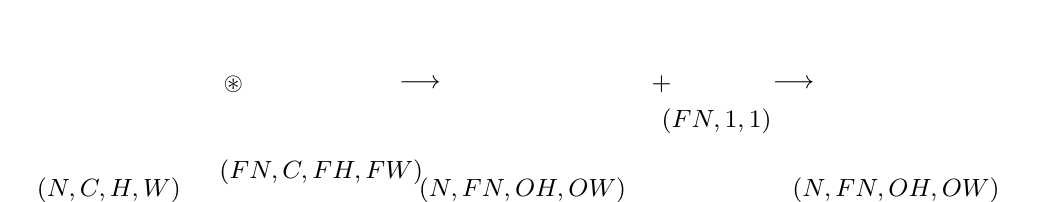
\begin{tikzpicture}[x=0.93cm,y=0.93cm]
\foreach \k in {2,1,0} {\cuboid{0.3*\k}{-0.25*\k}{1.4}{1.4}{0.8}{blue}}
\node[font=\small,below] at (0.95,-0.55) {$(N,C,H,W)$};
\node[font=\small] at (2.65,0.6) {$\circledast$};
\foreach \k in {3,2,1,0} {\cuboid{3.1+0.25*\k}{0.35-0.2*\k}{0.7}{0.7}{0.6}{blue}}
\node[font=\small,below] at (3.85,-0.3) {$(FN,C,FH,FW)$};
\node[font=\small] at (5.2,0.6) {$\longrightarrow$};
\foreach \k in {2,1,0} {\cuboid{5.8+0.3*\k}{-0.25*\k}{1.1}{1.1}{0.7}{orange}}
\node[font=\small,below] at (6.6,-0.55) {$(N,FN,OH,OW)$};
\node[font=\small] at (8.5,0.6) {$+$};
\cuboid{9.0}{0.45}{0.25}{0.25}{0.7}{orange}
\node[font=\small,below] at (9.25,0.4) {$(FN,1,1)$};
\node[font=\small] at (10.3,0.6) {$\longrightarrow$};
\foreach \k in {2,1,0} {\cuboid{10.9+0.3*\k}{-0.25*\k}{1.1}{1.1}{0.7}{orange}}
\node[font=\small,below] at (11.7,-0.55) {$(N,FN,OH,OW)$};
\end{tikzpicture}

\small 합성곱 연산의 배치 처리. $N$개의 데이터에 대한 합성곱을 한 번에 한다.
\end{center}

신경망에는 4차원 데이터가 하나 흐를 때마다 데이터 $N$개에 대한 합성곱 연산이 이루어진다.

% =================================================
\section{풀링 계층}\label{sec:pool}
% =================================================

\textbf{풀링(pooling)}은 세로, 가로 방향의 공간을 줄이는 연산이다.
아래는 $2\times2$ \textbf{최대 풀링(max pooling)}을 스트라이드 $2$로 하는 예이다.
$2\times2$ 영역마다 가장 큰 원소 하나를 꺼낸다.

\begin{center}
\begin{tikzpicture}
\fill[orange!30] (0,0) rectangle ({2*\cellsz},{-2*\cellsz});
\fill[blue!15] ({2*\cellsz},0) rectangle ({4*\cellsz},{-2*\cellsz});
\fill[green!20] (0,{-2*\cellsz}) rectangle ({2*\cellsz},{-4*\cellsz});
\fill[black!10] ({2*\cellsz},{-2*\cellsz}) rectangle ({4*\cellsz},{-4*\cellsz});
\numgrid{0}{0}{4}{1,2,1,0,0,1,2,3,3,0,1,2,2,4,0,1}
\draw[very thick] (0,0) rectangle ({4*\cellsz},{-4*\cellsz});
\draw[very thick] ({2*\cellsz},0) -- ({2*\cellsz},{-4*\cellsz});
\draw[very thick] (0,{-2*\cellsz}) -- ({4*\cellsz},{-2*\cellsz});
\node[font=\Large] at (3,-1) {$\longrightarrow$};
\fill[orange!30] (3.8,-0.5) rectangle ++(\cellsz,-\cellsz);
\fill[blue!15] ({3.8+\cellsz},-0.5) rectangle ++(\cellsz,-\cellsz);
\fill[green!20] (3.8,{-0.5-\cellsz}) rectangle ++(\cellsz,-\cellsz);
\fill[black!10] ({3.8+\cellsz},{-0.5-\cellsz}) rectangle ++(\cellsz,-\cellsz);
\numgrid{3.8}{-0.5}{2}{2,3,4,2}
\node[font=\small,below] at (1,-2.1) {입력 $(4,4)$};
\node[font=\small,below] at (4.3,-2.1) {출력 $(2,2)$};
\end{tikzpicture}
\end{center}

풀링의 윈도우 크기와 스트라이드는 보통 같은 값으로 한다 (윈도우 $3\times3$이면 스트라이드 $3$).
최대 풀링 외에 영역의 평균을 내는 \textbf{평균 풀링(average pooling)}도 있지만,
이미지 인식에서는 주로 최대 풀링을 쓴다. 이 노트에서 풀링이라 하면 최대 풀링을 뜻한다.

\begin{keybox}[풀링 계층의 특징]
\begin{itemize}[leftmargin=1.5em]
\item \textbf{학습해야 할 매개변수가 없다.} 영역에서 최댓값(또는 평균)을 취하는 명확한 처리일 뿐이다.
\item \textbf{채널 수가 변하지 않는다.} 채널마다 독립적으로 계산한다: $(N,C,H,W)\to(N,C,OH,OW)$.
\item \textbf{입력의 작은 변화에 영향을 적게 받는다(robust).}
입력이 한두 칸 이동해도 영역 안의 최댓값은 그대로인 경우가 많다.
\end{itemize}
\end{keybox}
\begin{lstlisting}
pool = Pooling(2, 2)                                    # max pooling, 2x2 window, stride 2
\end{lstlisting}
\begin{lstlisting}[language={},numbers=none]
2x2 max pooling:
 [[2. 3.]
 [4. 2.]]
\end{lstlisting}

% =================================================
\section{합성곱 / 풀링 계층 구현하기}\label{sec:impl}
% =================================================

지금까지 그래 왔듯이 합성곱 계층과 풀링 계층도 \texttt{forward}와 \texttt{backward}를 가진 클래스로 구현한다.
코드는 \texttt{code/conv\_layers.py}에 있고, Affine, ReLU, Softmax 계층은 지난 시간의 \texttt{layers.py}를 그대로 쓴다.

\begin{center}
\begin{tabular}{@{}p{0.3\textwidth}p{0.64\textwidth}@{}}
\toprule
파일 & 내용 \\
\midrule
\texttt{conv\_layers.py} & \texttt{im2col}, \texttt{col2im}, \texttt{Convolution}, \texttt{Pooling}, \texttt{Flatten}, \texttt{SimpleConvNet} \\
\texttt{layers.py}, \texttt{optimizers.py}, \texttt{mnist\_data.py} & 지난 시간의 모듈 (그대로 복사) \\[2pt]
\texttt{conv\_basics.py} & 이 노트의 예제, im2col 확인과 속도 비교, gradient 확인 \\
\texttt{mnist\_cnn.py} & SimpleConvNet으로 MNIST 학습, 필터와 특징 맵 시각화 \\
\texttt{mnist\_cnn\_torch.py} & 같은 network를 PyTorch로 \\
\bottomrule
\end{tabular}
\end{center}

\subsection{4차원 배열}\label{sec:4d}

CNN에서 계층 사이를 흐르는 데이터는 4차원 배열 $(N,C,H,W)$이다.
예를 들어 높이 $28$, 너비 $28$, 채널 $1$인 데이터가 $10$개라면 shape은 $(10,1,28,28)$이다.
\begin{lstlisting}[language={},numbers=none]
>>> x = np.random.rand(10, 1, 28, 28)
>>> x[0].shape         # the first image: (1, 28, 28)
>>> x[0, 0].shape      # its first channel: (28, 28)
\end{lstlisting}
지금까지 MNIST를 $(N,784)$로 다루었지만, CNN에서는 \texttt{reshape}으로 모양을 되살려 입력한다 (\texttt{mnist\_cnn.py}).
\begin{lstlisting}
x_train, t_train, x_val, t_val, x_test, t_test = load_mnist_split()
# a CNN keeps the SHAPE of the image: (N, 784) -> (N, 1, 28, 28) = (images, channels, height, width)
x_train = x_train.reshape(-1, 1, 28, 28)
\end{lstlisting}

\subsection{im2col로 데이터 전개하기}\label{sec:im2col}

합성곱을 \ref{sec:convop}절의 \texttt{conv2d\_naive}처럼 반복문으로 구현하면,
데이터 $N$개, 필터 $FN$개, 출력의 모든 위치 $OH\times OW$에 대하여 \texttt{for} 문이 겹겹이 필요하다.
numpy에서 \texttt{for} 문은 느리다. 그래서 \textbf{im2col}(image to column)이라는 함수로
입력 데이터를 필터를 적용하기 좋게 \textbf{2차원 행렬로 펼친다}.

\begin{keybox}[im2col의 아이디어]
필터가 방문하는 위치 하나마다, 그 위치의 입력 영역 $(C,FH,FW)$을 \textbf{한 행}으로 펼친다.
\begin{itemize}[leftmargin=1.5em]
\item 입력 $(N,C,H,W)$ $\xrightarrow{\text{im2col}}$ 행렬 $(N\cdot OH\cdot OW,\ C\cdot FH\cdot FW)$
\item 필터 $(FN,C,FH,FW)$ $\xrightarrow{\text{reshape}}$ 필터 하나를 \textbf{한 열}로: $(C\cdot FH\cdot FW,\ FN)$
\item 합성곱 $=$ 두 행렬의 곱 $+$ 편향: $(N\cdot OH\cdot OW,\ FN)$ $\xrightarrow{\text{reshape}}$ $(N,FN,OH,OW)$
\end{itemize}
\end{keybox}

\begin{center}
\begin{tikzpicture}[>=Latex]
% input with two windows
\cuboid{0}{0}{1.8}{1.8}{0.6}{blue}
\filldraw[fill=orange!50,draw=orange!80!black,thick] (0,1.8) rectangle ++(0.9,-0.9);
\filldraw[fill=green!40,draw=green!50!black,thick] (0.45,1.8) rectangle ++(0.9,-0.9);
\node[font=\scriptsize] at (0.3,1.1) {\ding{172}};
\node[font=\scriptsize] at (1.2,1.1) {\ding{173}};
\node[font=\small,below] at (0.9,-0.05) {입력 $(C,H,W)$};
\draw[->,thick] (2.5,0.8) -- node[above,font=\small] {im2col} (3.5,0.8);
% the column matrix: one row per filter position
\fill[orange!50] (3.7,2.0) rectangle (5.7,1.75);
\fill[green!40] (3.7,1.75) rectangle (5.7,1.5);
\draw[thick] (3.7,2.0) rectangle (5.7,-0.4);
\node[font=\scriptsize,anchor=east] at (3.65,1.875) {\ding{172}};
\node[font=\scriptsize,anchor=east] at (3.65,1.625) {\ding{173}};
\node[font=\small] at (4.7,0.6) {$\vdots$};
\node[font=\small,below,align=center] at (4.7,-0.45) {$(OH\cdot OW,$\\$C\cdot FH\cdot FW)$};
% the filters: one column per filter
\node[font=\Large] at (6.05,0.8) {$\cdot$};
\fill[blue!25] (6.4,2.0) rectangle (6.7,-0.4);
\fill[blue!45] (6.7,2.0) rectangle (7.0,-0.4);
\draw[thick] (6.4,2.0) rectangle (7.6,-0.4);
\node[font=\small,below,align=center] at (7.0,-0.45) {$(C\cdot FH\cdot FW,$\\$FN)$};
\node[font=\Large] at (8.1,0.8) {$=$};
\fill[orange!50] (8.6,2.0) rectangle (9.8,1.75);
\fill[green!40] (8.6,1.75) rectangle (9.8,1.5);
\draw[thick] (8.6,2.0) rectangle (9.8,-0.4);
\node[font=\small,below,align=center] at (9.2,-0.45) {$(OH\cdot OW,$\\$FN)$};
\draw[->,thick] (10.0,0.8) -- node[above,font=\small] {reshape} (11.2,0.8);
\cuboid{11.4}{0.2}{1.1}{1.1}{0.6}{orange}
\node[font=\small,below] at (11.95,0.15) {$(FN,OH,OW)$};
\end{tikzpicture}

\small im2col을 이용한 합성곱 (데이터 하나의 경우). 필터의 위치 \ding{172}, \ding{173}, $\ldots$이 행렬의 각 행이 된다.
\end{center}

이렇게 하면 합성곱 계층의 순전파는 \textbf{Affine 계층과 똑같은} 행렬곱 $A=\text{col}\cdot W_{\text{col}}+B$가 된다.
행렬곱은 numpy가 최적화된 선형대수 라이브러리(BLAS)로 계산하므로 매우 빠르다.
\begin{lstlisting}
def im2col(X, FH, FW, stride=1, pad=0):
    """(N, C, H, W) -> (N*OH*OW, C*FH*FW): ONE ROW for every place the filter visits"""
    N, C, H, W = X.shape
    OH, OW = output_size(H, FH, stride, pad), output_size(W, FW, stride, pad)
    Xp = np.pad(X, [(0, 0), (0, 0), (pad, pad), (pad, pad)])    # zero padding
    col = np.zeros((N, C, FH, FW, OH, OW))
    for i in range(FH):                   # loop over the FILTER, not the image
        for j in range(FW):
            col[:, :, i, j, :, :] = Xp[:, :, i:i + stride * OH:stride, j:j + stride * OW:stride]
    return col.transpose(0, 4, 5, 1, 2, 3).reshape(N * OH * OW, -1)
\end{lstlisting}
반복문은 이미지 전체가 아니라 \textbf{필터의 크기} ($FH\times FW$, 예: $5\times5=25$번)만큼만 돈다.
\texttt{(i, j)} 번째 반복에서는 ``필터의 $(i,j)$ 원소와 곱해질 입력의 값들''을 모든 출력 위치에 대해 한꺼번에 잘라 온다.
마지막 \texttt{transpose}와 \texttt{reshape}으로 출력 위치마다 한 행이 되도록 정리한다.
\begin{lstlisting}
x1 = np.random.rand(1, 3, 7, 7)                         # 1 image, 3 channels, 7x7
print("im2col of (1, 3, 7, 7) with a 5x5 filter:", im2col(x1, 5, 5).shape)
x2 = np.random.rand(10, 3, 7, 7)                        # 10 images
print("im2col of (10, 3, 7, 7) with a 5x5 filter:", im2col(x2, 5, 5).shape)
\end{lstlisting}
\begin{lstlisting}[language={},numbers=none]
im2col of (1, 3, 7, 7) with a 5x5 filter: (9, 75)
im2col of (10, 3, 7, 7) with a 5x5 filter: (90, 75)
\end{lstlisting}
$7\times7$ 입력에 $5\times5$ 필터를 적용하면 출력은 $3\times3=9$개의 위치이고,
각 위치의 입력 영역은 $3\times5\times5=75$개의 값이다. 데이터가 $10$개이면 행이 $90$개가 된다.

\paragraph{얼마나 빠를까?}
MNIST 크기의 미니배치 $(100,1,28,28)$에 $5\times5$ 필터 $30$개를 적용하는 합성곱을,
네 겹의 반복문과 im2col로 각각 계산해 비교한다.
\begin{lstlisting}
def conv_loops(X, W, B):
    """(N, C, H, W) with FN filters (FN, C, FH, FW): every image, every filter, every position"""
    N, C, H, Wd = X.shape
    FN, _, FH, FW = W.shape
    OH, OW = H - FH + 1, Wd - FW + 1
    Y = np.zeros((N, FN, OH, OW))
    for n in range(N):
        for k in range(FN):
            for i in range(OH):
                for j in range(OW):
                    Y[n, k, i, j] = np.sum(X[n, :, i:i + FH, j:j + FW] * W[k]) + B[k]
    return Y
\end{lstlisting}
\begin{lstlisting}[language={},numbers=none]
output shape (100, 30, 24, 24), max |difference| = 5.3e-15
loops 5.74 s,  im2col 0.057 s  (101 times faster)
\end{lstlisting}
결과는 같고 (차이 $10^{-15}$), im2col이 약 $100$배 빠르다.
반복문으로는 미니배치 하나에 $6$초가 걸리므로, $550$개의 미니배치로 이루어진 한 epoch에 거의 $1$시간이 걸린다.

\begin{remarkbox}[im2col의 대가: 메모리]
필터가 겹쳐서 이동하면 입력의 같은 값이 im2col 행렬의 여러 행에 중복해서 들어간다.
$(100,1,28,28)$ 입력 ($78400$개의 값)이 $5\times5$ 필터로 전개되면
$(100\cdot24\cdot24,\ 25)=(57600,25)$, 즉 $144$만 개의 값이 된다. 약 $18$배이다.
메모리를 더 쓰는 대신 속도를 얻는 것이다.
그래서 \texttt{SimpleConvNet}의 \texttt{accuracy}는 $10000$장을 한꺼번에 넣지 않고 $1000$장씩 나누어 계산한다.
GPU용 라이브러리(cuDNN 등)는 im2col 외에도 FFT, Winograd 같은 여러 방법을 상황에 따라 골라 쓴다.
\end{remarkbox}

\subsection{합성곱 계층 구현하기}\label{sec:convlayer}

im2col을 쓰면 합성곱 계층의 순전파는 ``im2col $\to$ Affine $\to$ reshape''이다.
\begin{lstlisting}
class Convolution:
    """Convolution of (N, C, H, W) with FN filters (FN, C, FH, FW) -> (N, FN, OH, OW).
       With im2col: ONE matrix product, i.e. an Affine layer at every filter position."""
    def __init__(self, W, B, stride=1, pad=0):
        self.W = W                  # (FN, C, FH, FW)
        self.B = B                  # (FN,): one bias per filter
        self.stride = stride
        self.pad = pad
        self.dW = None
        self.dB = None

    def forward(self, X):
        FN, C, FH, FW = self.W.shape
        N, _, H, W = X.shape
        OH = output_size(H, FH, self.stride, self.pad)
        OW = output_size(W, FW, self.stride, self.pad)
        self.X_shape = X.shape
        self.col = im2col(X, FH, FW, self.stride, self.pad)     # (N*OH*OW, C*FH*FW)
        self.W_col = self.W.reshape(FN, -1).T                    # one filter per COLUMN
        A = self.col @ self.W_col + self.B                       # (N*OH*OW, FN)
        return A.reshape(N, OH, OW, FN).transpose(0, 3, 1, 2)    # (N, FN, OH, OW)
\end{lstlisting}
\texttt{A}의 각 행은 (데이터, 출력 위치) 하나, 각 열은 필터(출력 채널) 하나이다.
그래서 \texttt{reshape(N, OH, OW, FN)}으로 나눈 뒤, 채널 축을 두 번째로 옮겨 $(N,FN,OH,OW)$를 만든다.
출력 크기는 \ref{sec:stride}절의 식을 그대로 함수로 만든 것이다.
\begin{lstlisting}
def output_size(H, FH, stride=1, pad=0):
    """height (or width) of the output: OH = (H + 2P - FH) / S + 1"""
    return (H + 2 * pad - FH) // stride + 1
\end{lstlisting}

\paragraph{합성곱 계층의 역전파.}
순전파가 세 단계로 나뉘었으므로, 변수 노드 기준의 계산 그래프로 그리면 다음과 같다.

\begin{center}
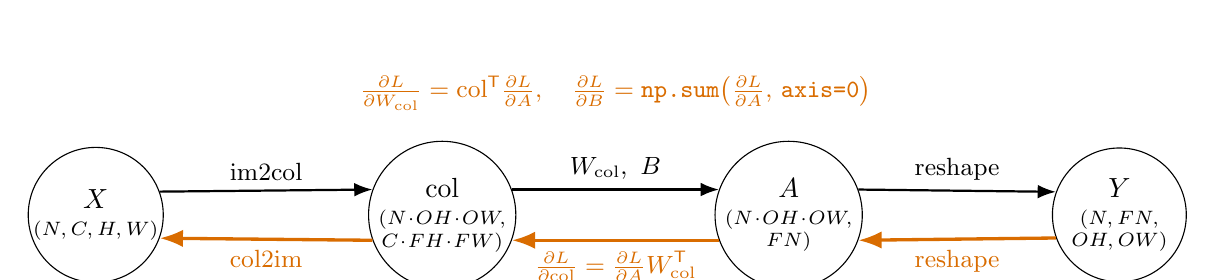
\begin{tikzpicture}[>=Latex,
  var/.style={draw,circle,minimum size=17mm,align=center,inner sep=0pt},
  bw/.style={<-,very thick,orange!85!black},
  bl/.style={orange!85!black,font=\small,align=center}]
\node[var] (X) at (0,0) {$X$\\[-2pt]{\scriptsize $(N,C,H,W)$}};
\node[var] (col) at (4.4,0) {col\\[-2pt]{\scriptsize $(N\!\cdot\!OH\!\cdot\!OW,$}\\[-4pt]{\scriptsize $C\!\cdot\!FH\!\cdot\!FW)$}};
\node[var] (A) at (8.8,0) {$A$\\[-2pt]{\scriptsize $(N\!\cdot\!OH\!\cdot\!OW,$}\\[-4pt]{\scriptsize $FN)$}};
\node[var] (Y) at (13.0,0) {$Y$\\[-2pt]{\scriptsize $(N,FN,$}\\[-4pt]{\scriptsize $OH,OW)$}};
\draw[->,thick] (X.20) -- node[above,font=\small] {im2col} (col.160);
\draw[->,thick] (col.20) -- node[above,font=\small] {$W_{\text{col}},\ B$} (A.160);
\draw[->,thick] (A.20) -- node[above,font=\small] {reshape} (Y.160);
\draw[bw] (X.-20) -- node[below,bl] {col2im} (col.-160);
\draw[bw] (col.-20) -- node[below,bl] {$\pd{L}{\text{col}}=\pd{L}{A}W_{\text{col}}\T$} (A.-160);
\draw[bw] (A.-20) -- node[below,bl] {reshape} (Y.-160);
\node[bl] at (6.6,1.55) {$\pd{L}{W_{\text{col}}}=\text{col}\T\pd{L}{A},\quad \pd{L}{B}=\texttt{np.sum}\bigl(\pd{L}{A},\,\texttt{axis=0}\bigr)$};
\end{tikzpicture}

\small 합성곱 계층의 계산 그래프. 가운데는 지난 시간의 Affine 계층 그대로이다.
\end{center}

\begin{itemize}[leftmargin=1.8em]
\item \textbf{reshape의 역전파}는 gradient의 모양을 원래대로 되돌리는 것뿐이다 (값은 그대로 전달).
\item \textbf{가운데는 Affine 계층}이다. 지난 시간에 유도한
$\pd{L}{W}=X\T\pd{L}{A}$, $\pd{L}{B}=\sum_{\text{행}}\pd{L}{A}$, $\pd{L}{X}=\pd{L}{A}W\T$를 그대로 쓴다.
\item \textbf{im2col의 역전파}는 \textbf{col2im}이다. im2col에서 입력의 한 값이 col의 여러 행에 복사되었으므로
(필터 위치가 겹치는 곳), 역전파에서는 그 값으로 돌아오는 gradient를 \textbf{모두 더해야} 한다.
한 변수에서 화살표가 여러 개 나가면 gradient를 더한다는 다변수 연쇄법칙(배치 정규화에서 보았다)과 같은 원리이다.
\end{itemize}

\begin{lstlisting}
    def backward(self, dA):
        FN, C, FH, FW = self.W.shape
        dA = dA.transpose(0, 2, 3, 1).reshape(-1, FN)            # (N*OH*OW, FN)
        self.dB = np.sum(dA, axis=0)                             # the Affine rules
        self.dW = (self.col.T @ dA).T.reshape(FN, C, FH, FW)
        dcol = dA @ self.W_col.T                                 # (N*OH*OW, C*FH*FW)
        return col2im(dcol, self.X_shape, FH, FW, self.stride, self.pad)
\end{lstlisting}
\begin{lstlisting}
def col2im(col, X_shape, FH, FW, stride=1, pad=0):
    """the reverse of im2col: ADD every row back where it came from"""
    N, C, H, W = X_shape
    OH, OW = output_size(H, FH, stride, pad), output_size(W, FW, stride, pad)
    col = col.reshape(N, OH, OW, C, FH, FW).transpose(0, 3, 4, 5, 1, 2)
    Xp = np.zeros((N, C, H + 2 * pad, W + 2 * pad))
    for i in range(FH):
        for j in range(FW):
            Xp[:, :, i:i + stride * OH:stride, j:j + stride * OW:stride] += col[:, :, i, j, :, :]
    return Xp[:, :, pad:pad + H, pad:pad + W]     # remove the padding
\end{lstlisting}
im2col에서 \texttt{=}로 잘라 온 자리에, col2im에서는 \texttt{+=}로 더해 넣는다는 것만 다르다.

\subsection{풀링 계층 구현하기}\label{sec:poollayer}

풀링 계층도 im2col로 입력을 전개한다. 다만 풀링은 \textbf{채널마다 독립적}이므로,
전개한 뒤 한 행이 ``한 채널의 한 윈도우''가 되도록 다시 \texttt{reshape}하고, 행마다 최댓값을 구한다.

\begin{center}
\begin{tikzpicture}
\fill[orange!30] (0,0) rectangle ({2*\cellsz},{-2*\cellsz});
\fill[blue!15] ({2*\cellsz},0) rectangle ({4*\cellsz},{-2*\cellsz});
\fill[green!20] (0,{-2*\cellsz}) rectangle ({2*\cellsz},{-4*\cellsz});
\fill[black!10] ({2*\cellsz},{-2*\cellsz}) rectangle ({4*\cellsz},{-4*\cellsz});
\numgrid{0}{0}{4}{1,2,1,0,0,1,2,3,3,0,1,2,2,4,0,1}
\node[font=\small] at (2.9,-1) {$\xrightarrow{\text{전개}}$};
\fill[orange!30] (3.6,0) rectangle ++({4*\cellsz},-\cellsz);
\fill[blue!15] (3.6,-\cellsz) rectangle ++({4*\cellsz},-\cellsz);
\fill[green!20] (3.6,{-2*\cellsz}) rectangle ++({4*\cellsz},-\cellsz);
\fill[black!10] (3.6,{-3*\cellsz}) rectangle ++({4*\cellsz},-\cellsz);
\numgrid{3.6}{0}{4}{1,2,0,1,1,0,2,3,3,0,2,4,1,2,0,1}
\node[font=\small] at (6.4,-1) {$\xrightarrow{\text{max}}$};
\numgrid{7.2}{0}{1}{2,3,4,2}
\node[font=\small] at (8.4,-1) {$\xrightarrow{\text{reshape}}$};
\numgrid{9.3}{-0.5}{2}{2,3,4,2}
\end{tikzpicture}

\small 풀링 계층의 구현: 윈도우마다 한 행으로 전개하고, 행마다 최댓값을 구한 뒤 모양을 되돌린다.
\end{center}

\begin{lstlisting}
    def forward(self, X):
        N, C, H, W = X.shape
        OH = output_size(H, self.PH, self.stride, self.pad)
        OW = output_size(W, self.PW, self.stride, self.pad)
        col = im2col(X, self.PH, self.PW, self.stride, self.pad)
        col = col.reshape(-1, self.PH * self.PW)           # one window per row
        self.argmax = np.argmax(col, axis=1)               # where the maximum was
        self.X_shape = X.shape
        Y = np.max(col, axis=1)
        return Y.reshape(N, OH, OW, C).transpose(0, 3, 1, 2)   # (N, C, OH, OW)
\end{lstlisting}

\paragraph{풀링 계층의 역전파.}
$y=\max(x_1,x_2,x_3,x_4)$에서 최댓값이 $x_k$이면 $\pd{y}{x_k}=1$이고 나머지는 $0$이다.
즉 최댓값이었던 원소에만 gradient를 그대로 전달하고, 나머지에는 $0$을 보낸다.
ReLU에서 \texttt{mask}로 통과한 원소에만 gradient를 보낸 것과 같다.
순전파에서 최댓값의 위치(\texttt{argmax})를 기억해 두는 이유이다.
\begin{lstlisting}
    def backward(self, dY):
        dY = dY.transpose(0, 2, 3, 1).ravel()               # the same order as col
        dcol = np.zeros((dY.size, self.PH * self.PW))
        dcol[np.arange(dY.size), self.argmax] = dY          # only the max gets it
        dcol = dcol.reshape(-1, self.X_shape[1] * self.PH * self.PW)
        return col2im(dcol, self.X_shape, self.PH, self.PW, self.stride, self.pad)
\end{lstlisting}

\subsection{Flatten 계층}\label{sec:flatten}

합성곱과 풀링을 거친 4차원 데이터를 Affine 계층에 넣으려면 데이터마다 한 줄로 펼쳐야 한다.
이것을 계층 하나로 만들어 둔다 (PyTorch의 \texttt{nn.Flatten}). 역전파는 모양을 되돌리는 것뿐이다.
\begin{lstlisting}
class Flatten:
    """(N, C, H, W) -> (N, C*H*W) before an Affine layer (nn.Flatten in PyTorch)"""
    def forward(self, X):
        self.X_shape = X.shape
        return X.reshape(X.shape[0], -1)

    def backward(self, dY):
        return dY.reshape(self.X_shape)
\end{lstlisting}

% =================================================
\section{CNN 구현하기}\label{sec:simplecnn}
% =================================================

합성곱 계층과 풀링 계층을 조합하여 손글씨 숫자를 인식하는 CNN을 만든다.
책의 \texttt{SimpleConvNet}과 같은 구조이다.

\begin{center}
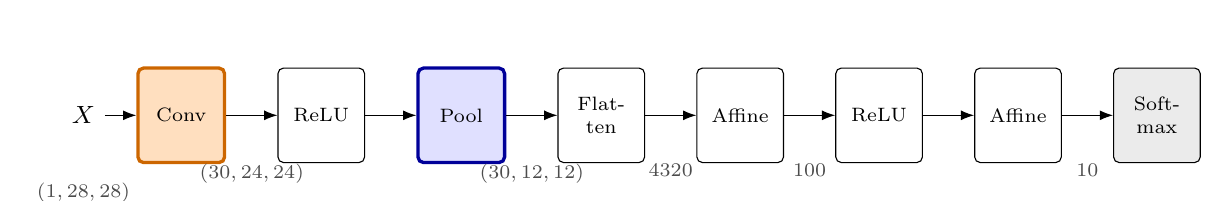
\begin{tikzpicture}[>=Latex,
  lay/.style={draw,rounded corners=2pt,minimum width=11mm,minimum height=12mm,
              font=\scriptsize,align=center,inner sep=1pt},
  cv/.style={lay,fill=orange!25,draw=orange!80!black,very thick},
  pl/.style={lay,fill=blue!12,draw=blue!60!black,very thick},
  sh/.style={font=\scriptsize,align=center,text=black!70},
  node distance=6.5mm]
\node[font=\small] (in) {$X$};
\node[cv,right=4mm of in] (c1) {Conv};
\node[lay,right=of c1] (r1) {ReLU};
\node[pl,right=of r1] (p1) {Pool};
\node[lay,right=of p1] (f1) {Flat-\\ten};
\node[lay,right=of f1] (a1) {Affine};
\node[lay,right=of a1] (r2) {ReLU};
\node[lay,right=of r2] (a2) {Affine};
\node[lay,right=of a2,fill=black!8] (sm) {Soft-\\max};
\draw[->] (in) -- (c1);
\draw[->] (c1) -- node[sh,below=5mm] {$(30,24,24)$} (r1);
\draw[->] (r1) -- (p1);
\draw[->] (p1) -- node[sh,below=5mm] {$(30,12,12)$} (f1);
\draw[->] (f1) -- node[sh,below=5mm] {$4320$} (a1);
\draw[->] (a1) -- node[sh,below=5mm] {$100$} (r2);
\draw[->] (r2) -- (a2);
\draw[->] (a2) -- node[sh,below=5mm] {$10$} (sm);
\node[sh,below=5mm] at (in.south) {$(1,28,28)$};
\end{tikzpicture}

\small SimpleConvNet의 구조와 각 계층을 지난 뒤 데이터 하나의 shape
\end{center}

\begin{center}
{\small
\begin{tabular}{@{}llcr@{}}
\toprule
계층 & 설정 & 출력 shape & 매개변수 수 \\
\midrule
입력 & & $(1,28,28)$ & \\
Conv & $5\times5$ 필터 $30$개 & $(30,24,24)$ & $30\cdot1\cdot5\cdot5+30=780$ \\
ReLU & & $(30,24,24)$ & \\
Pooling & $2\times2$ 최대 풀링 & $(30,12,12)$ & \\
Flatten & & $4320$ & \\
Affine & & $100$ & $4320\cdot100+100=432100$ \\
ReLU & & $100$ & \\
Affine & & $10$ & $100\cdot10+10=1010$ \\
\midrule
합계 & & & $433890$ \\
\bottomrule
\end{tabular}}

(합성곱은 스트라이드 $1$, 패딩 $0$, 풀링은 스트라이드 $2$이다. 출력 shape은 데이터 하나의 것이다.)
\end{center}

합성곱 계층의 매개변수는 $780$개뿐이고, 매개변수의 $99.6\%$는 첫 번째 Affine 계층에 있다.
합성곱 계층이 가중치를 공유하기 때문이다 (\ref{sec:blocks}절).

\texttt{SimpleConvNet}은 지난 시간의 \texttt{MultiLayerNet}과 같은 방식으로 만든다.
매개변수를 \texttt{params} 딕셔너리에 두고, 같은 배열을 계층에도 넘겨주어
optimizer가 \texttt{params}를 갱신하면 계층의 가중치도 바뀌게 한다. 초깃값은 He 초깃값이다.
합성곱 필터 하나가 보는 입력의 수는 $C\cdot FH\cdot FW=25$개이므로 표준편차는 $\sqrt{2/25}$이다.
\begin{lstlisting}
class SimpleConvNet:
    """Conv -> ReLU -> Pool -> Flatten -> Affine -> ReLU -> Affine -> Softmax"""
    def __init__(self, input_shape=(1, 28, 28), filter_num=30, filter_size=5,
                 hidden_size=100, output_size=10):
        C, H, W = input_shape
        conv_out = H - filter_size + 1                     # 28 - 5 + 1 = 24
        pool_out = conv_out // 2                           # 2x2 max pooling: 12
        flat = filter_num * pool_out * pool_out            # 30 * 12 * 12 = 4320
        n_in = C * filter_size * filter_size               # 25 inputs per filter
        self.params = {                                    # He initialization
            "W1": np.sqrt(2.0 / n_in) * np.random.randn(filter_num, C, filter_size, filter_size),
            "B1": np.zeros(filter_num),
            "W2": np.sqrt(2.0 / flat) * np.random.randn(flat, hidden_size),
            "B2": np.zeros((1, hidden_size)),
            "W3": np.sqrt(2.0 / hidden_size) * np.random.randn(hidden_size, output_size),
            "B3": np.zeros((1, output_size)),
        }
        self.layers = [
            Convolution(self.params["W1"], self.params["B1"]),
            Relu(),
            Pooling(2, 2),
            Flatten(),
            Affine(self.params["W2"], self.params["B2"]),
            Relu(),
            Affine(self.params["W3"], self.params["B3"]),
        ]
        self.last = SoftmaxWithCrossEntropy()
\end{lstlisting}
순전파, 손실, 역전파는 \texttt{MultiLayerNet}과 똑같다.
계층이 모두 같은 \texttt{forward}, \texttt{backward} 형식을 따르기 때문에,
새로운 계층이 들어와도 network 코드는 바뀌지 않는다. 이것이 계층 단위로 구현하는 장점이다.
\begin{lstlisting}
    def backward(self):                       # call right after loss()
        d = self.last.backward()
        for layer in reversed(self.layers):   # layer after layer
            d = layer.backward(d)
        grads, k = {}, 0
        for layer in self.layers:
            if isinstance(layer, (Convolution, Affine)):
                k += 1
                grads[f"W{k}"], grads[f"B{k}"] = layer.dW, layer.dB
        return grads
\end{lstlisting}

\paragraph{gradient 확인.}
작은 \texttt{SimpleConvNet} (입력 $(2,8,8)$, $3\times3$ 필터 $3$개)으로 역전파와 수치미분을 비교한다
(\texttt{conv\_basics.py}의 (3)).
\begin{lstlisting}
np.random.seed(1)
small = SimpleConvNet(input_shape=(2, 8, 8), filter_num=3, filter_size=3, hidden_size=5, output_size=4)
X_small = np.random.randn(5, 2, 8, 8)                   # 5 images, 2 channels, 8x8
T_small = np.eye(4)[np.random.randint(0, 4, size=5)]
small.loss(X_small, T_small)
grads = small.backward()
\end{lstlisting}
\begin{lstlisting}[language={},numbers=none]
W1: shape (3, 2, 3, 3)    max |backprop - numerical| = 1.15e-09
B1: shape (3,)            max |backprop - numerical| = 1.22e-09
W2: shape (27, 5)         max |backprop - numerical| = 1.42e-09
B2: shape (1, 5)          max |backprop - numerical| = 6.68e-10
W3: shape (5, 4)          max |backprop - numerical| = 1.03e-09
B3: shape (1, 4)          max |backprop - numerical| = 3.82e-10
\end{lstlisting}
합성곱, 풀링, Flatten을 지나는 역전파가 모두 올바르다.

\paragraph{MNIST로 학습하기.}
\texttt{mnist\_cnn.py}에서 \texttt{SimpleConvNet}을 Adam (학습률 $0.001$, 미니배치 $100$)으로 $10$ epoch 학습시킨다.
비교를 위해 지난 시간의 다층 퍼셉트론(MLP, $784\to100\to10$, He 초깃값)도 같은 조건으로 학습시킨다.
\begin{lstlisting}
np.random.seed(1)
cnn = SimpleConvNet(input_shape=(1, 28, 28), filter_num=30, filter_size=5,
                    hidden_size=100, output_size=10)
print("SimpleConvNet parameters:", cnn.num_params())
W1_before = cnn.params["W1"].copy()                   # the filters before training
cnn_result = train(cnn)
\end{lstlisting}

\IfFileExists{figures/cnn_mnist.png}{%
\begin{center}
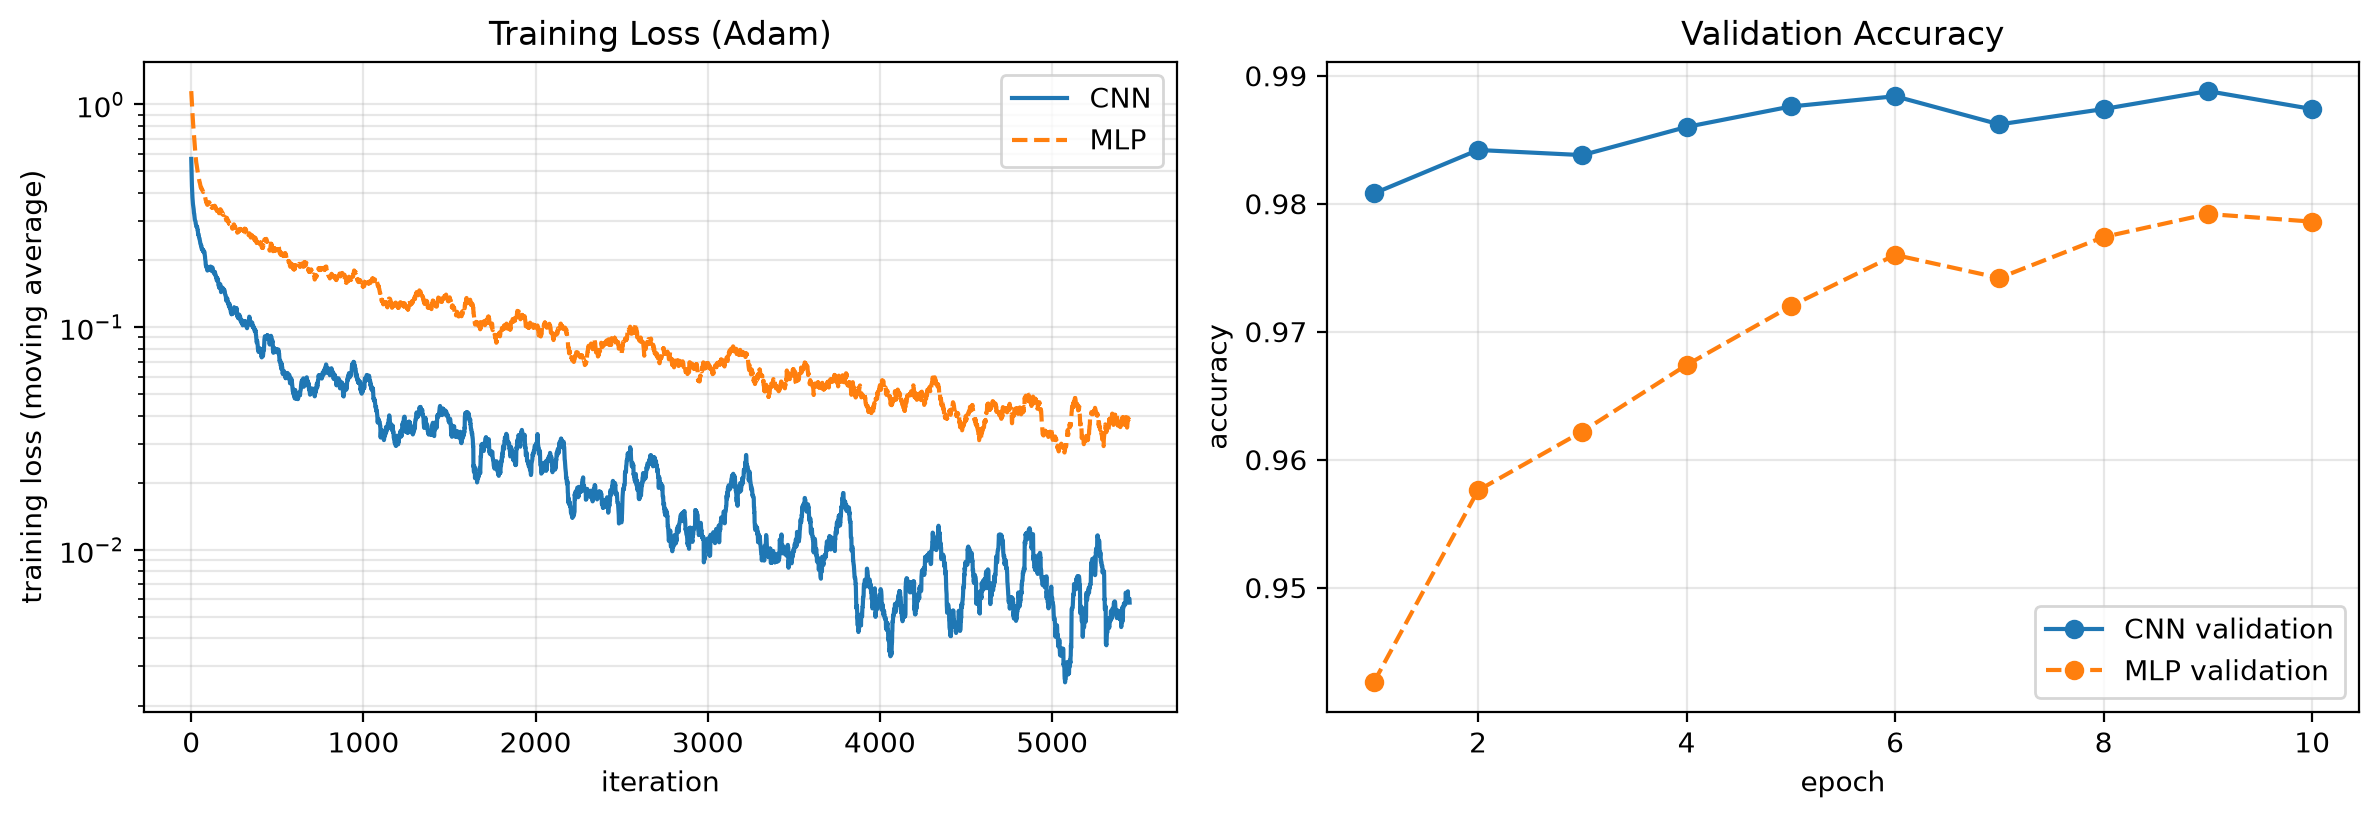
\includegraphics[width=\textwidth]{figures/cnn_mnist.png}

\small SimpleConvNet과 MLP의 훈련 손실 (50 iteration 이동평균, 로그 눈금, 왼쪽)과 epoch별 검증 정확도 (오른쪽)
\end{center}
}{%
\begin{center}
\fbox{\parbox{0.8\textwidth}{\centering\small
[그림 자리] \texttt{figures/cnn\_mnist.png}\\
\texttt{mnist\_cnn.py}를 실행하면 생성된다.}}
\end{center}
}

\begin{center}
{\small
\begin{tabular}{@{}lccccccc@{}}
\toprule
& \multicolumn{4}{c}{검증 정확도} & & & \\
\cmidrule(lr){2-5}
& 1 epoch & 2 epoch & 5 epoch & 10 epoch & 시험 & 매개변수 & epoch당 \\
\midrule
SimpleConvNet & $98.1\%$ & $98.4\%$ & $98.8\%$ & $98.7\%$ & $\mathbf{98.6\%}$ & $433890$ & 약 $60$초 \\
MLP ($784\to100\to10$) & $94.3\%$ & $95.8\%$ & $97.2\%$ & $97.9\%$ & $97.6\%$ & $79510$ & 약 $1$초 \\
\bottomrule
\end{tabular}}
\end{center}

\begin{itemize}[leftmargin=1.8em]
\item CNN은 \textbf{첫 epoch 만에} 검증 정확도 $98.1\%$로, MLP가 $10$ epoch 동안 도달한 $97.9\%$보다 높다.
시험 정확도는 $98.6\%$로 MLP보다 $1\%$p 높다. 틀리는 수로 보면 $10000$장 중 $237$장에서 $145$장으로 약 $40\%$ 줄었다.
\item 손실도 CNN이 훨씬 빨리, 훨씬 낮게 내려간다.
\item 다만 매개변수 수가 다르므로 공정한 비교는 아니다. CNN의 매개변수 대부분은 합성곱 계층이 아니라 Affine 계층에 있다.
합성곱 계층의 $780$개 매개변수가 이미지의 모양을 이용해 \textbf{좋은 특징}을 만들어 주기 때문에
뒤의 Affine 계층이 분류를 더 쉽게 하는 것이다.
\item numpy로 구현한 CNN은 한 epoch에 약 $1$분이 걸린다. 합성곱은 계산량이 많아 GPU와 최적화된 라이브러리가 중요하다.
\end{itemize}

책에서는 $20$ epoch 학습하여 시험 정확도 약 $99\%$를 얻는다.
이 노트에서는 시간을 줄이려고 $10$ epoch만 학습하였다.

% =================================================
\section{CNN 시각화하기}\label{sec:visual}
% =================================================

CNN의 합성곱 계층은 무엇을 보고 있을까? 학습된 필터와 그 출력을 그려 본다.

\subsection{첫 번째 층의 가중치 시각화하기}\label{sec:filters}

첫 번째 합성곱 계층의 필터는 $(30,1,5,5)$, 즉 $5\times5$ 크기의 흑백 이미지 $30$장으로 볼 수 있다.
학습 전과 후의 필터를 이미지로 그리면 다음과 같다 (밝을수록 큰 가중치).

\IfFileExists{figures/cnn_filters.png}{%
\begin{center}
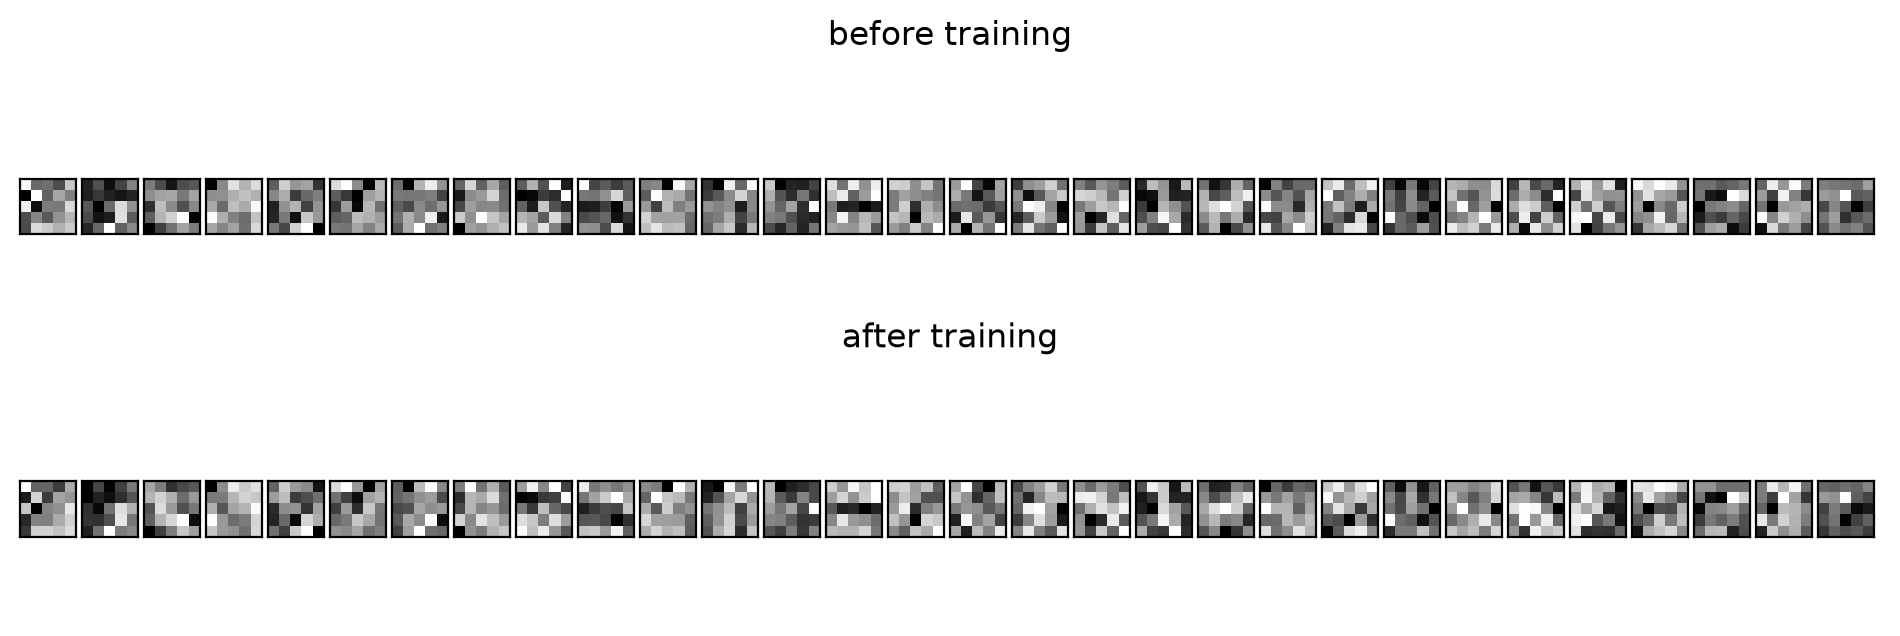
\includegraphics[width=\textwidth]{figures/cnn_filters.png}

\small 첫 번째 합성곱 계층의 필터 $30$개: 학습 전 (위)과 학습 후 (아래)
\end{center}
}{%
\begin{center}
\fbox{\parbox{0.8\textwidth}{\centering\small
[그림 자리] \texttt{figures/cnn\_filters.png}\\
\texttt{mnist\_cnn.py}를 실행하면 생성된다.}}
\end{center}
}

책의 그림에서는 학습 전에는 무작위였던 필터가 학습 후에는 흰색과 검은색이 규칙적으로 나뉜 모양으로 바뀐다.
그런데 우리 결과에서는 학습 전과 후의 필터가 \textbf{비슷해 보인다}.
초깃값의 차이 때문이다. 책은 표준편차 $0.01$의 아주 작은 값에서 시작하므로 학습된 부분이 그대로 드러나지만,
우리는 He 초깃값 (표준편차 $\sqrt{2/25}\approx0.28$)에서 시작하였고, 학습률 $0.001$인 Adam으로 $10$ epoch 동안
필터가 바뀐 양은 처음 값에 비해 크지 않다. 처음의 무작위 무늬가 많이 남아 있는 것이다.
그래도 이 필터들로 검증 정확도 $98.7\%$를 얻었다.
무작위에 가까운 필터도 서로 다른 방향의 에지를 어느 정도 잡아내고, 학습이 그것을 조금씩 다듬은 것이다.

\paragraph{필터는 무엇에 반응하는가: 특징 맵.}
필터 자체보다 필터를 이미지에 적용한 결과, 즉 \textbf{특징 맵}을 보면 필터의 역할이 더 잘 드러난다.
학습된 network의 합성곱 계층에 시험 이미지 하나를 넣어 출력 $(1,30,24,24)$ 중 앞의 $8$장을 그린다.
\begin{lstlisting}
image = x_test[:1]                                     # (1, 1, 28, 28)
feature = cnn.layers[0].forward(image)                 # (1, 30, 24, 24)
\end{lstlisting}

\IfFileExists{figures/cnn_feature_maps.png}{%
\begin{center}
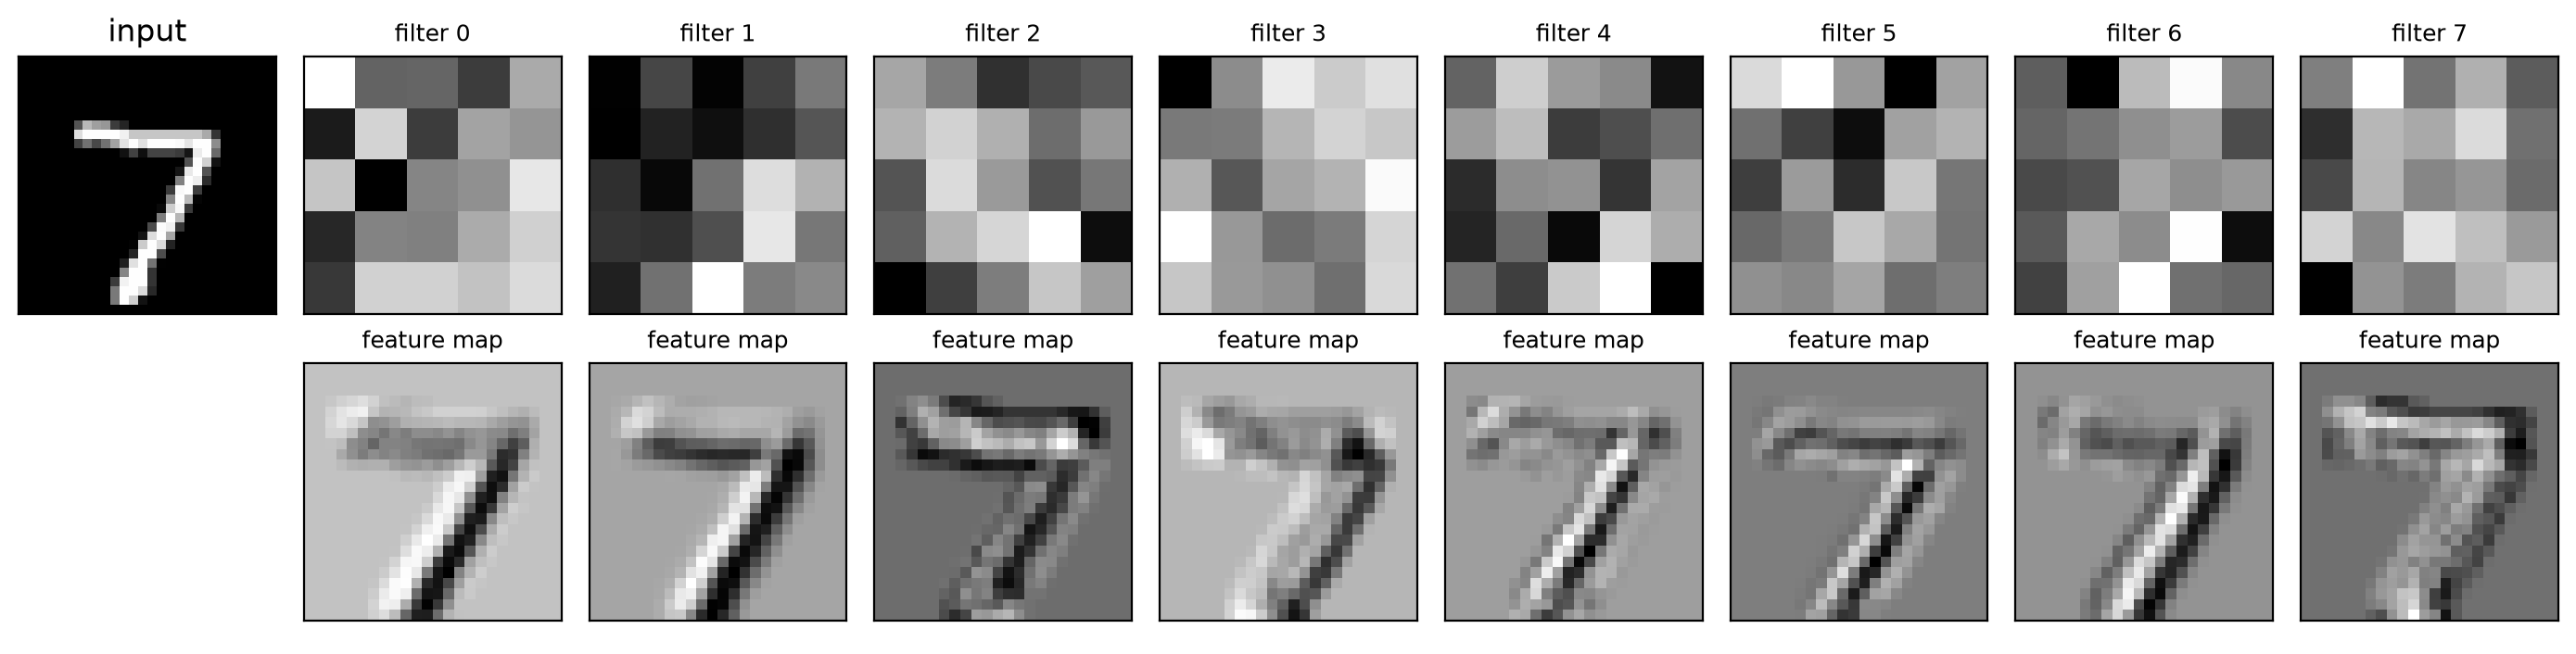
\includegraphics[width=\textwidth]{figures/cnn_feature_maps.png}

\small 입력 이미지와 학습된 필터 $8$개 (위), 각 필터의 출력 특징 맵 (아래, ReLU 적용 전)
\end{center}
}{%
\begin{center}
\fbox{\parbox{0.8\textwidth}{\centering\small
[그림 자리] \texttt{figures/cnn\_feature\_maps.png}\\
\texttt{mnist\_cnn.py}를 실행하면 생성된다.}}
\end{center}
}

\begin{itemize}[leftmargin=1.8em]
\item 특징 맵마다 숫자 7의 \textbf{서로 다른 부분이 밝게}(큰 값) 나타난다.
예를 들어 필터 $0$과 $1$은 대각선 획의 한쪽 가장자리에서 밝고 반대쪽 가장자리에서 어둡다.
필터 $2$는 위쪽 가로 획의 가장자리에 강하게 반응한다.
\item 즉 첫 번째 층의 필터는 특정 방향의 \textbf{에지}(색이 바뀌는 경계)에 반응한다.
같은 필터를 모든 위치에 적용하므로, 그 방향의 에지가 이미지의 어디에 있든 찾아낸다.
\item 이렇게 만든 $30$장의 특징 맵을 풀링으로 줄인 뒤 Affine 계층이 조합하여 숫자를 판단한다.
\end{itemize}

\subsection{층 깊이에 따른 추출 정보 변화}\label{sec:depth}

첫 번째 층의 필터는 에지나 블롭(blob, 국소적으로 덩어리진 영역) 같은 \textbf{저수준 정보}에 반응한다.
그렇다면 층을 여러 개 쌓으면 어떻게 될까?
Zeiler와 Fergus (2014) 등의 연구에서 대규모 이미지 데이터로 학습한 깊은 CNN의 각 층이 무엇에 반응하는지 시각화한 결과,
층이 깊어질수록 더 복잡하고 추상적인 정보가 추출된다는 것이 알려졌다.

\begin{center}
\begin{tikzpicture}[>=Latex,
  st/.style={draw,rounded corners=3pt,fill=orange!12,draw=orange!70!black,minimum width=26mm,minimum height=11mm,align=center,font=\small},
  node distance=5mm]
\node[st] (l1) {에지, 블롭\\(edge, blob)};
\node[st,right=of l1] (l2) {텍스처\\(texture)};
\node[st,right=of l2] (l3) {사물의 일부\\(object parts)};
\node[st,right=of l3] (l4) {사물 전체\\(클래스)};
\draw[->,thick] (l1) -- (l2);
\draw[->,thick] (l2) -- (l3);
\draw[->,thick] (l3) -- (l4);
\node[font=\small,below=2mm of l1] {앞쪽 층};
\node[font=\small,below=2mm of l4] {뒤쪽 층};
\end{tikzpicture}

\small 깊은 CNN에서 층이 깊어질수록 뉴런이 반응하는 대상
\end{center}

앞쪽 층은 단순한 모양에, 중간 층은 그것들을 조합한 무늬와 부분에, 뒤쪽 층은 사물 전체에 반응한다.
이렇게 \textbf{단순한 특징을 조합하여 점점 추상적인 특징을 만드는 것}이 층을 깊게 쌓는 이유이다.
합성곱 계층을 여러 번 거칠수록 출력의 한 원소가 보는 입력의 범위(\textbf{수용 영역, receptive field})가 넓어지므로,
뒤쪽 층일수록 이미지의 넓은 영역을 보고 판단할 수 있다.

% =================================================
\section{대표적인 CNN}\label{sec:famous}
% =================================================

CNN의 원조인 LeNet과, 딥러닝이 주목받게 된 계기가 된 AlexNet을 살펴본다.

\subsection{LeNet}\label{sec:lenet}

LeNet은 손글씨 숫자를 인식하는 network로 1998년에 제안되었다 (LeCun 등).
합성곱 계층과 풀링 계층(정확히는 원소를 줄이기만 하는 \textbf{서브샘플링} 계층)을 반복하고,
마지막으로 완전연결 계층을 거쳐 결과를 출력한다.

\begin{center}
\begin{tikzpicture}[>=Latex,
  lay/.style={draw,rounded corners=2pt,minimum width=12mm,minimum height=11mm,font=\scriptsize,align=center,inner sep=1pt},
  cv/.style={lay,fill=orange!25,draw=orange!80!black,very thick},
  pl/.style={lay,fill=blue!12,draw=blue!60!black,very thick},
  sh/.style={font=\scriptsize,align=center,text=black!70},
  node distance=6mm]
\node[sh] (in) {입력\\$32\times32$};
\node[cv,right=of in] (c1) {Conv\\$5\times5$};
\node[pl,right=of c1] (s2) {Sub-\\sampling};
\node[cv,right=of s2] (c3) {Conv\\$5\times5$};
\node[pl,right=of c3] (s4) {Sub-\\sampling};
\node[lay,right=of s4] (f5) {FC};
\node[lay,right=of f5] (f6) {FC};
\node[lay,right=of f6] (out) {출력};
\draw[->] (in) -- (c1);
\draw[->] (c1) -- node[sh,above=5mm] {$6@28\times28$} (s2);
\draw[->] (s2) -- node[sh,below=5mm] {$6@14\times14$} (c3);
\draw[->] (c3) -- node[sh,above=5mm] {$16@10\times10$} (s4);
\draw[->] (s4) -- node[sh,below=5mm] {$16@5\times5$} (f5);
\draw[->] (f5) -- node[sh,above=5mm] {$120$} (f6);
\draw[->] (f6) -- node[sh,below=5mm] {$84$} (out);
\node[sh,right=1mm of out] {$10$};
\end{tikzpicture}

\small LeNet의 구조. ``$6@28\times28$''은 $28\times28$ 크기의 특징 맵 $6$장이라는 뜻이다.
\end{center}

\texttt{SimpleConvNet}과 비교하면 거의 같은 구조이지만, 지금의 CNN과는 다음이 다르다.
\begin{itemize}[leftmargin=1.8em]
\item \textbf{활성화 함수}: LeNet은 sigmoid 계열의 함수 (scaled tanh)를 썼다. 지금은 주로 ReLU를 쓴다.
\item \textbf{풀링}: LeNet은 서브샘플링으로 중간 데이터의 크기를 줄였다. 지금은 최대 풀링이 주류이다.
\end{itemize}
그래도 거의 $30$년 전에 이미 지금의 CNN과 같은 기본 구조가 완성되어 있었다는 것이 놀라운 점이다.

\subsection{AlexNet}\label{sec:alexnet}

LeNet 이후 오랫동안 주목받지 못하던 CNN은 2012년 AlexNet (Krizhevsky, Sutskever, Hinton)의 등장으로
딥러닝 열풍을 일으켰다. 대규모 이미지 인식 대회(ILSVRC 2012)에서 top-5 오류율 약 $15\%$로,
$26\%$였던 2위와 큰 차이로 우승하였다.

\begin{center}
\resizebox{\textwidth}{!}{%
\begin{tikzpicture}[>=Latex,
  lay/.style={draw,rounded corners=2pt,minimum width=11mm,minimum height=11mm,font=\scriptsize,align=center,inner sep=1pt},
  cv/.style={lay,fill=orange!25,draw=orange!80!black,very thick},
  pl/.style={lay,fill=blue!12,draw=blue!60!black,very thick},
  sh/.style={font=\scriptsize,align=center,text=black!70},
  node distance=3.2mm]
\node[sh] (in) {입력\\$224\times224$\\$\times3$};
\node[cv,right=of in] (c1) {Conv\\$11\times11$\\$96$};
\node[pl,right=of c1] (p1) {Pool};
\node[cv,right=of p1] (c2) {Conv\\$5\times5$\\$256$};
\node[pl,right=of c2] (p2) {Pool};
\node[cv,right=of p2] (c3) {Conv\\$3\times3$\\$384$};
\node[cv,right=of c3] (c4) {Conv\\$3\times3$\\$384$};
\node[cv,right=of c4] (c5) {Conv\\$3\times3$\\$256$};
\node[pl,right=of c5] (p3) {Pool};
\node[lay,right=of p3] (f1) {FC\\$4096$};
\node[lay,right=of f1] (f2) {FC\\$4096$};
\node[lay,right=of f2] (f3) {FC\\$1000$};
\foreach \u/\v in {in/c1,c1/p1,p1/c2,c2/p2,p2/c3,c3/c4,c4/c5,c5/p3,p3/f1,f1/f2,f2/f3}
  \draw[->] (\u) -- (\v);
\node[sh,below=2mm of c1] {$55\times55$};
\node[sh,below=2mm of c2] {$27\times27$};
\node[sh,below=2mm of c4] {$13\times13$};
\node[sh,below=2mm of p3] {$6\times6$};
\end{tikzpicture}}

\small AlexNet의 구조: 합성곱 계층 $5$개와 완전연결 계층 $3$개. 아래 숫자는 특징 맵의 크기이다.
\end{center}

AlexNet은 합성곱 계층과 풀링 계층을 거듭하며 마지막으로 완전연결 계층을 거쳐 결과를 출력한다는 점에서 LeNet과 같지만,
다음과 같은 변화가 있었다.
\begin{itemize}[leftmargin=1.8em]
\item 활성화 함수로 \textbf{ReLU}를 쓴다.
\item LRN(Local Response Normalization)이라는 국소적 정규화를 하는 계층을 쓴다
(지금은 배치 정규화로 대체되었다).
\item \textbf{드롭아웃}을 쓴다 (완전연결 계층).
\item 최대 풀링을 쓴다.
\end{itemize}
매개변수는 약 $6000$만 개이다. 이것을 학습할 수 있었던 것은 네트워크 구조뿐 아니라
\textbf{빅데이터}(ImageNet, 약 $120$만 장의 학습 이미지)와 대량의 병렬 계산을 하는 \textbf{GPU}가 보급된 덕분이다.

\begin{keybox}[AlexNet에는 지금까지 배운 부품이 모두 있다]
ReLU, 최대 풀링, 드롭아웃 (지난 주), 정규화 계층 (배치 정규화의 선배 격), GPU에서의 대규모 행렬곱 (im2col).
그 뒤의 CNN도 같은 부품을 더 깊게 쌓는 방향으로 발전하였다:
VGG (2014, $3\times3$ 합성곱만 $16\sim19$층), GoogLeNet (2014, 여러 크기의 필터를 병렬로),
ResNet (2015, 입력을 건너뛰어 더하는 skip connection으로 $150$층 이상).
\end{keybox}

% =================================================
\section{PyTorch로 구현하기}\label{sec:torchcnn}
% =================================================

지난 시간에 PyTorch로 완전연결 network를 만들었다.
같은 방법으로 \texttt{SimpleConvNet}을 PyTorch로 만들면, 바뀌는 것은 계층의 이름뿐이다
(\texttt{mnist\_cnn\_torch.py}).
\begin{center}
\begin{tabular}{@{}ll@{}}
\toprule
우리의 구현 (\texttt{conv\_layers.py}) & PyTorch \\
\midrule
\texttt{Convolution(W, B, stride, pad)} & \texttt{nn.Conv2d(C, FN, kernel\_size, stride, padding)} \\
\texttt{Pooling(2, 2)} & \texttt{nn.MaxPool2d(2)} \\
\texttt{Flatten()} & \texttt{nn.Flatten()} \\
필터 \texttt{W}: $(FN,C,FH,FW)$ & \texttt{weight}: $(FN,C,FH,FW)$ (같은 순서) \\
\bottomrule
\end{tabular}
\end{center}
\begin{lstlisting}
model = nn.Sequential(
    nn.Conv2d(1, 30, kernel_size=5),      # (N, 1, 28, 28) -> (N, 30, 24, 24)
    nn.ReLU(),
    nn.MaxPool2d(2),                      # -> (N, 30, 12, 12)
    nn.Flatten(),                         # -> (N, 4320)
    nn.Linear(30 * 12 * 12, 100),
    nn.ReLU(),
    nn.Linear(100, 10),
).to(device)
\end{lstlisting}
데이터는 $(N,1,28,28)$ 모양의 텐서로 만들어 넣는다. 학습 루프는 지난 시간의 코드와 같다.
\begin{lstlisting}
def to_dataset(x, t):
    """images (N, 784) -> (N, 1, 28, 28) tensors, one-hot labels -> class indices"""
    return TensorDataset(torch.tensor(x, dtype=torch.float32).reshape(-1, 1, 28, 28),
                         torch.tensor(np.argmax(t, axis=1)))
\end{lstlisting}

\begin{center}
\begin{tabular}{@{}lcccccc@{}}
\toprule
& \multicolumn{4}{c}{검증 정확도} & & \\
\cmidrule(lr){2-5}
& 1 epoch & 2 epoch & 5 epoch & 10 epoch & 시험 & epoch당 \\
\midrule
numpy (\texttt{conv\_layers.py}) & $98.1\%$ & $98.4\%$ & $98.8\%$ & $98.7\%$ & $98.6\%$ & 약 $60$초 \\
PyTorch (CPU) & $97.6\%$ & $98.4\%$ & $98.6\%$ & $99.1\%$ & $98.8\%$ & 약 $12$초 \\
\bottomrule
\end{tabular}
\end{center}

\begin{itemize}[leftmargin=1.8em]
\item 같은 구조, 같은 optimizer이므로 결과가 비슷하다. 초깃값과 미니배치 순서가 다르므로 숫자가 똑같지는 않다.
\item 같은 CPU에서 PyTorch가 약 $5$배 빠르다. PyTorch는 합성곱을 C++로 최적화된 라이브러리로 계산하며,
GPU가 있으면 \texttt{device="cuda"}만으로 수십 배 더 빨라진다.
\item PyTorch의 \texttt{nn.Conv2d}는 기본 초깃값이 He 초깃값보다 작다 (균등분포, 범위 $\pm1/\sqrt{25}$).
그래서 학습된 필터에 학습으로 생긴 무늬가 더 잘 드러난다. 여러 방향의 에지 모양을 볼 수 있다.
\end{itemize}

\IfFileExists{figures/cnn_torch_filters.png}{%
\begin{center}
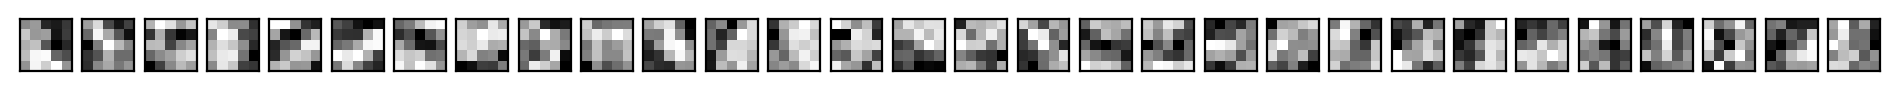
\includegraphics[width=\textwidth]{figures/cnn_torch_filters.png}

\small PyTorch로 학습한 첫 번째 합성곱 계층의 필터 $30$개 (\texttt{model[0].weight})
\end{center}
}{%
\begin{center}
\fbox{\parbox{0.8\textwidth}{\centering\small
[그림 자리] \texttt{figures/cnn\_torch\_filters.png}\\
\texttt{mnist\_cnn\_torch.py}를 실행하면 생성된다.}}
\end{center}
}

% =================================================
\section{정리}\label{sec:summary}
% =================================================

\begin{keybox}[합성곱 신경망: 정리]
\begin{itemize}[leftmargin=1.5em]
\item CNN은 지금까지의 신경망에 \textbf{합성곱 계층}과 \textbf{풀링 계층}을 더한 것이다.
\item 합성곱 계층은 이미지의 \textbf{형상을 유지}하며, 같은 필터를 모든 위치에 적용한다 (가중치 공유).
출력 크기는 $OH=\frac{H+2P-FH}{S}+1$.
\item 필터는 4차원 $(FN,C,FH,FW)$, 데이터는 4차원 $(N,C,H,W)$이다.
\item 풀링 계층은 매개변수 없이 공간 크기를 줄이며, 작은 위치 변화에 강하다.
\item \textbf{im2col}을 쓰면 합성곱은 하나의 행렬곱, 즉 Affine 계층이 된다. 역전파는 Affine의 역전파와 col2im이다.
\item 첫 층의 필터는 에지와 블롭에 반응하고, 층이 깊어질수록 더 추상적인 정보를 추출한다.
\item LeNet (1998)과 AlexNet (2012)이 대표적인 CNN이며, 빅데이터와 GPU가 딥러닝 발전의 큰 원동력이었다.
\end{itemize}
\end{keybox}

% =================================================
\section{연습문제}
% =================================================

\begin{enumerate}[label=\arabic*.]

\item 다음 합성곱 계층의 출력 크기를 구하라.
(a) 입력 $(32,32)$, 필터 $(5,5)$, 패딩 $2$, 스트라이드 $1$.
(b) 입력 $(227,227)$, 필터 $(11,11)$, 패딩 $0$, 스트라이드 $4$ (AlexNet의 첫 번째 층).
(c) 입력 $(28,28)$에 $2\times2$ 최대 풀링 (스트라이드 $2$)을 두 번 적용한 결과.

\item 입력 $\begin{pmatrix}1&0&2&1\\0&3&1&0\\2&1&0&4\\1&0&1&2\end{pmatrix}$에
필터 $\begin{pmatrix}1&0\\0&-1\end{pmatrix}$를 스트라이드 $1$, 패딩 $0$으로 적용한 결과를 손으로 계산하라.
같은 입력에 $2\times2$ 최대 풀링을 적용한 결과도 구하라.

\item RGB 이미지 ($C=3$)에 $3\times3$ 필터 $64$개를 쓰는 합성곱 계층의 매개변수(가중치와 편향) 수를 구하라.
입력이 $(3,32,32)$이고 패딩 $1$일 때, 같은 크기의 출력 $(64,32,32)$을 완전연결 계층으로 만든다면 가중치는 몇 개가 필요한가?

\item 2번 문제의 최대 풀링에서 출력 쪽 gradient가 $\begin{pmatrix}1&2\\3&4\end{pmatrix}$일 때,
입력 쪽 gradient ($4\times4$)를 구하라.

\item 길이 $5$인 1차원 입력 $(x_1,\ldots,x_5)$에 길이 $3$인 필터를 스트라이드 $1$로 적용하면 출력은 $3$개이다.
im2col 행렬 ($3\times3$)을 쓰고, $x_3$이 몇 번 등장하는지 세어 보라.
이로부터 col2im에서 gradient를 \textbf{더해야} 하는 이유를 설명하라.

\item SimpleConvNet의 합성곱 계층에 패딩 $2$를 주도록 고쳐 보라.
\texttt{conv\_out}, \texttt{pool\_out}, \texttt{flat}은 각각 얼마가 되는가?
Convolution 계층에 \texttt{pad}를 넘기는 부분과 \texttt{flat}의 계산을 고친 뒤,
\texttt{conv\_basics.py}의 gradient 확인으로 검증하라.

\item \texttt{mnist\_cnn\_torch.py}를 고쳐 LeNet과 비슷한 network
(Conv $5\times5$ $6$개, 패딩 $2$ $\to$ ReLU $\to$ MaxPool $\to$ Conv $5\times5$ $16$개 $\to$ ReLU $\to$ MaxPool $\to$ FC $120$ $\to$ FC $84$ $\to$ FC $10$)를 만들고 학습시켜라.
각 계층을 지난 뒤의 shape을 표로 정리하고, 매개변수 수와 검증 정확도를 SimpleConvNet과 비교하라.

\end{enumerate}

\end{document}
